\documentclass[english,notitlepage,reprint,nofootinbib]{revtex4-2}  % defines the basic parameters of the document
% For preview: skriv i terminal: latexmk -pdf -pvc filnavn
% If you want a single-column, remove "reprint"
\setlength{\parindent}{0pt}
\setlength{\parskip}{7pt}

% Allows special characters (including æøå)
\usepackage[utf8]{inputenc}
\usepackage[english]{babel}

\usepackage{physics,amssymb}  % mathematical symbols (physics imports amsmath)
%\include{amsmath}
\usepackage{graphicx}         % include graphics such as plots
\usepackage{xcolor}           % set colors
\usepackage{hyperref}         % automagic cross-referencing
\usepackage{url}
\usepackage{listings}         % display code
\usepackage{subfigure}        % imports a lot of cool and useful figure commands
\usepackage{caption}
%\usepackage{subcaption} % for subfigures, also imports caption package
\usepackage{float}
\usepackage{nicematrix}
\usepackage{multirow}
%\usepackage[section]{placeins}
%\usepackage[left=1.5cm, right=1.5cm]{geometry}
\usepackage{algorithm}
\usepackage[noend]{algpseudocode}
\usepackage{tikz}
\usetikzlibrary{quantikz}
\usepackage{algorithm}
%\usepackage[noend]{algpseudocode}
\usepackage[style=numeric, backend=bibtex, sorting=none]{biblatex}
\addbibresource{sources.bib}
\usepackage{authblk}
% defines the color of hyperref objects
% Blending two colors:  blue!80!black  =  80% blue and 20% black
\hypersetup{ % this is just my personal choice, feel free to change things
    colorlinks,
    linkcolor={red!50!black},
    citecolor={blue!50!black},
    urlcolor={blue!80!black}}
    
%\bibliographystyle{unsrtnat}  
\bibliographystyle{apsrev4-2}
\newcommand{\ditto}{%
    \tikz{
        \draw [line width=0.12ex] (-0.2ex,0) -- +(0,0.8ex)
            (0.2ex,0) -- +(0,0.8ex);
        \draw [line width=0.08ex] (-0.6ex,0.4ex) -- +(-1.5em,0)
            (0.6ex,0.4ex) -- +(1.5em,0);
    }%
}
% So that we use same notation from the start:
% Reference with "Eq. \label{..}", "Fig.", "Sec."
% External references/sources should be put in ref.bib and referenced with \cite{...}
% code and other code-related things should be inside \texttt{}
% British English

    
\begin{document}
% Deadline October 7 

\title{\vspace*{-2cm}\bf Classification using a Feed-Forward Neural Network \hspace*{5cm}\makebox[-5cm]{\includegraphics[width=0.13\linewidth]{UiO_Segl_300dpi.png}}\\
FYS-STK4155\\
\rule{\textwidth}{0.05cm}}
\author[1]{Oskar Hafstad}
\author[3]{Simon H. Hille}
\author[1, 2]{Semya A. Tønnessen}
% self-explanatory
\affil[1]{Institute for Theoretical Astrophysics, University of Oslo}
\affil[2]{Center for Computing in Science Education, University of Oslo}
\affil[3]{Department of Physics, University of Cologne}
\date{\today}
%\noaffiliation
\begin{abstract} \centering Link to Github repo: \url{https://github.com/hafos/FYS-STK4155/project2}% Remember to use short and direct formulations!
\vspace{3mm}
\\
In this project, our aim is to investigate classification and regression problems using a Feed-Forward Neural Network (FFNN). We will compare this method this to linear and logistic regression whilst studying two data sets: The Franke function and the Wisconsin Breast Cancer data set. 
The goal is to study which methods are best with regards to computational time and accuracy. 
Our results show that the neural networks code is better suited to the classification problem, achieving a higher accuracy than our logistic regression code and scikit learn's logistic regression function. Meanwhile, for the regression problem the logistic regression code performed slightly better. Various activation functions point towards the Sigmoid function producing the best results in this case, but the logistic regression code still performed better. 

The implementation and material relevant to this project can be found at the Github repo referenced above. 
\end{abstract}
\maketitle

\section{Introduction} 
% The main purpose of the introduction section is to provide context and motivation for the work. It is also common --- and quite useful --- to use the last paragraph of the introduction to outline the rest of the report, to tell the reader what they should expect in the different sections.

% Motivate what we do 
The field of artificial neural networks has a long history of development, starting with McCulloch and Pitts developing a model of artificial neurons in in 1943 in order to study signal processing in the brain. As computer science and computers themselves become more advanced, the field of artificial neural networks has been refined and will continue to advance~\cite{lecture_notes}. Today, it is used in many technological fields, from medicine where trained models can assist in diagnostic and treatment decisions, to providing entertainment companies with models for what products a costumer is more likely to consume. 
\vspace{3mm}
\\
The neural nets are neural-inspired nonlinear models for supervised learning, which attempt to mimic the neural networks of an animal brain, composed of billions of neurons that communicate by sending electrical signals. The signals must exceed a threshold in order to yield output, or else the neuron remains inactive. 
The method offers a simple way of analyzing large amounts of data when an exact model is not applicable, and it is often used within regression and classification problems. Neural nets can be viewed as natural, more powerful extensions of supervised learning methods such as linear and logistic regression and soft-max methods~\cite{lecture_notes}. 
\vspace{3mm}
\\
% It is vital to properly communicate precisely what has been done, what the results are and their implications. The motivation for this is to make the work understood and reproducible, so that others can both check and build on your work.
The aim of this project is to study classification and regression problems by developing our own Feed-Forward Neural Network (FFNN) in python. 
In order to analyze the efficiency and accuracy of each method, we compute the Mean-Squared Error (MSE) and accuracy score. 
\vspace{3mm}
\\
Previously, we analyzed and developed algorithms for two linear regression methods which we will make use of in this project: The Ordinary Least Square (OLS) method and Ridge regression. We will also include logistic regression for classification problems and write an algorithm for the FFNN for studying both regression and classification problems. 
\vspace{3mm}
\\
In section \ref{sec:methods} we provide a short summary of the linear regression methods we use, OLS and Ridge regression, as well as an overview of logistic regression and gradient descent. Additionally, we explain relevant theory behind the FFNN and present the datasets we will be working with. 
A selection of results relevant to our understanding are presented together with a discussion of the results in section~\ref{sec:results}, 
%A selection of results relevant to our understanding are presented in section \ref{sec:results}. In section \ref{sec:discussion} we discuss how our results correspond to our expectations, 
and in section~\ref{sec:conclusion} we provide a short summary and outlook. 


%\section{Theory}                    % (optional) 
%_______________________________METHOD___________________________________________
\section{Method}\label{sec:methods}

\subsection*{Linear and Logistic Regression}
When using linear regression we approximate a function $f(\boldsymbol{x})$ by $\Tilde{\boldsymbol{y}} = \mathbf{X}\boldsymbol{\beta}$, where the matrix $\mathbf{X}$ is the design matrix and $\boldsymbol{\beta}$ are the unknown parameters we want to determine. 
The model is fitted by finding the values of $\boldsymbol{\beta}$ which minimize the cost function $C(\mathbf{X}, \boldsymbol{\beta}$) where the cost function is a function which allows us to judge how well the model $\boldsymbol{\beta}$ fits the matrix $\mathbf{X}$. The minimum is usually found using numerical methods, as analytical methods are generally not possible. 
\vspace{3mm}
\\
A common linear regression model is the ordinary least squared (OLS), where we assume a cost function 
% defined from the mean squared error
\begin{align}\label{eq: costfunc_OLS}
    \mathcal{C}_\text{OLS}(\boldsymbol{\beta}) = \frac{1}{n}\left\{(\boldsymbol{y} - \mathbf{X}\boldsymbol{\beta})^T (\boldsymbol{y} - \mathbf{X}\boldsymbol{\beta})\right\},
\end{align}
which, when minimized, yields the OLS expression for the optimal parameter $\hat{\boldsymbol{\beta}}$. 
Another common model is Ridge regression, where we include a regularization parameter $\lambda$, and for which the cost function becomes 
% weighted mse 
\begin{align}\label{eq: costfunc_ridge}
    C(\mathbf{X},\boldsymbol{\beta})_\text{Ridge} = \left\{ (\boldsymbol{y} - \mathbf{X}\boldsymbol{\beta})^T (\boldsymbol{y} - \mathbf{X}\boldsymbol{\beta}) \right\} + \lambda\boldsymbol{\beta}^T\boldsymbol{\beta}. 
\end{align}
For the linear regression analysis our main interest was around leading the coefficients of a functional fit in order to be able to predict the response of a continuous variable on some unseen data. 
% The fit to the continuous variable y_i is based on some independent variables x_i. 
Linear regression resulted in analytical expressions for standard OLS or Ridge regression for several quantities, ranging from the variance and thereby the confidence intervals of the parameters $\beta$ to the mean squared error (MSE)~\cite{lecture_notes}. By inverting the product of the design matrices we could fit our data. 
\vspace{3mm}
\\
Classification problems, on the other hand, are concerned with outcomes which take the form of discrete variables. 
Obtaining such a discrete output can be done by using the perceptron model, which is a "hard classification" model where each data point is deterministically assigned to a category. In many cases, however, it is favorable to use a "soft classifier" that outputs the probability of a given category rather than a single value, which is where we apply logistic regression. 
\vspace{3mm}
\\
When we apply logistic regression the most common situation is having two possible outcomes, normally denoted as a binary outcome~\cite{lecture_notes}. 
The probability that a data point $x_i$ belongs to a category $y_i = \{0,1\}$ is given by the logistic function, also known as the Sigmoid function, 
\begin{align}\label{eq: logistic_function} % sigmoid function
    p(t) = \frac{1}{1+\exp -t} = \frac{\exp t}{1+\exp t}, 
\end{align}
which is meant to represent the likelihood of a given event~\cite{lecture_notes}. 
Assuming that we have two categories with $y_i\in\{0,1\}$ and that we only have two parameters $\beta$ in the fit of the Sigmoid function, we define the probabilities 
\begin{align}
    p(y_i=1 | x_i,\boldsymbol{\beta}) &= 
    \frac{\exp(\beta_0 + \beta_1 x_i)}
    {1 + \exp(\beta_0 + \beta_1 x_i)} \\ 
    p(y_i=0 | x_i,\boldsymbol{\beta}) &= 
    1 - p(y_i=1 | x_i,\boldsymbol{\beta}) , 
\end{align}
where $x$ is an input set and $\boldsymbol{\beta}$ are the weights we wish to extract from data, in this case $\beta_0$ and $\beta_1$ which are the coefficients we use to estimate the data. 
\vspace{3mm}
\\ 
Our aim is now to maximize the probability of seeing the observed data. 
Using the Maximum Likelihood Estimation (MLE), we define the total likelihood for all possible outcomes from a dataset $\mathcal{D} = \{(y_i,x_i)\}$ with the binary labels $y_i\in\{0,1\}$: 
\begin{align}
    P(\mathcal{D}|\boldsymbol{\beta}) 
    = \prod\limits_{i=1}^n 
    [p(y_i=1|x_i,\boldsymbol{\beta})]^{y_i}
    [1 - p(y_i=1|x_i,\boldsymbol{\beta})]^{1-y_i}, 
\end{align}
which then is an approximation of the likelihood in terms of the individual probabilities of a specific outcome $y_i$~\cite{lecture_notes}. 
From this we obtain the log-likelihood
\begin{align}
    \mathcal{C}(\boldsymbol{\beta}) 
    &= \sum\limits_{i=1}^n (y_i 
    \log p(y_i=1|x_i,\boldsymbol{\beta}) \nonumber \\ 
    &+ (1-y_i) 
    \log[1 - p(y_i=1|x_i,\boldsymbol{\beta})]), 
\end{align}
which is a cost function. 
The maximum likelihood estimator is defined as the set of parameters that maximize the log-likelihood where we maximize with respect to $\beta$. The cost function is the negative log-likelihood, and so by reordering the logarithms, it can be rewritten as 
\begin{align}\label{eq: cost function logistic regression}
    C(\boldsymbol{\beta}) = -\sum\limits_{i=1}^n (y_i(\beta_0 + \beta_1 x_i) - \log(1+\exp(\beta_0 + \beta_1 x_i))).
\end{align}
This cost function, known as cross entropy, is what we use for logistic regression, and it is often supplemented with additional regularization terms. 
\vspace{3mm}
\\ 
We minimize the cross entropy cost function with respect to the two parameters $\beta_0$ and $\beta_1$, keeping in mind that this is a convex function of the weights $\boldsymbol{\beta}$, thereby making any local minimizer a global minimizer. By defining a vector $\boldsymbol{y}$ with $n$ elements $y_i$, an $n\times p$ matrix $\mathbf{X}$ which contains the $x_i$ values and a vector $\boldsymbol{p}$ of fitted probabilities $p(y_i | x_i, \boldsymbol{\beta})$, we find that the first derivative of the cost function becomes 
\begin{align}
    \frac{\partial \mathcal{C}(\boldsymbol{\beta})}{\partial \boldsymbol{\beta}} = -\boldsymbol{X}^T\left(\boldsymbol{y}-\boldsymbol{p}\right).
\end{align}
By defining a diagonal matrix $\mathbf{W}$ with elements $p(y_i | x_i, \boldsymbol{\beta})(1 - p(y_i | x_i, \boldsymbol{\beta}))$, we obtain an expression for the second derivative 
\begin{align}
    \frac{\partial^2 \mathcal{C}(\boldsymbol{\beta})}{\partial \boldsymbol{\beta}\partial \boldsymbol{\beta}^T} = \boldsymbol{X}^T\boldsymbol{W}\boldsymbol{X}.
\end{align}
\vspace{3mm}
\\ 
In order to measure the performance of the classification problem we will use the accuracy score, which is the number of correctly guessed targets $t_i$ divided by the total number of targets $n$, 
\begin{align}
    \text{Accuracy} = \frac{\sum_{i=1}^n I(t_i = y_i)}{n}, 
\end{align}
where $I$ is the indicator function, $1$ if $t_i = y_i$ and $0$ otherwise for a binary classification problem. 
\vspace{3mm}
\\ 
When performing the linear regression analysis we solved for the best value for $\boldsymbol{\beta}$ by taking the inverse. However, this is not always possible, and in such cases we can apply a method which takes advantage of numerical optimization, called gradient descent. 

\subsection*{Gradient Methods}
% a) We replace the matrix inversion algorithm in the OLS and Ridge regression with a gradient descent (GD) and SGD codes. 
Previously, we have solved OLS and Ridge regression using an algorithm for matrix inversion. 
We now study another method for minimizing a function $\boldsymbol{f}(\boldsymbol{x})$. 
\vspace{3mm}
\\ 
Gradient descent, also known as Steepest Descent, is an optimization algorithm we use in order to find the minima of $\boldsymbol{f}(\boldsymbol{x})$, where $\boldsymbol{x} = (x_1, ..., x_n$). A function such as this is expected to decrease fastest while going from $x$ towards the direction of the negative gradient $-\Delta\boldsymbol{f}(\boldsymbol{x})$. 

The method can be used in the training of a machine learning model, where it is applied to the convex cost function in order to minimize this to its local minimum. 
For a certain amount of iterative steps towards the direction of the minima, we will eventually reach a point where the cost function is at its smallest if 
\begin{align}
    \boldsymbol{x}_{k+1} = \boldsymbol{x}_k - \gamma_k \Delta\boldsymbol{f}(\boldsymbol{x}_k), \nonumber 
\end{align}
where the step length/learning rate $\gamma_k > 0$. If $\gamma_k$ is sufficiently small we are always moving towards smaller function values, $\boldsymbol{f}(\boldsymbol{x}_{k+1} \leq \boldsymbol{f}(\boldsymbol{x}_k))$. 

Ideally the sequence $\{\boldsymbol{x}_k\}_{k=0}$ converges towards a global minimum of the function $\boldsymbol{f}$, and this is always the case when $\boldsymbol{f}$ is a convex function, as all local minima are also global minima. While this scheme is simple and straightforward to implement, it has several limitations such as being sensitive to the chosen initial condition and being expensive to compute numerically.

The gradient descent method is sensitive to the choice of learning rate $\gamma_k$, due to the fact that we require a sufficiently small $\gamma_k$ to reach the minima. Choosing a learning rate that is too small leads to the method taking a long time to converge, while choosing a too large learning rate can lead to erratic behaviour. 

\subsubsection*{Stochastic Gradient Descent}%__________________________________________
Many of these shortcomings can be alleviated by introducing randomness. One such method is that of Stochastic Gradient Descent (SGD). 
\vspace{3mm}
\\ 
The cost function, which we want to minimize, can often be written as a sum over $n$ data points $\{\boldsymbol{x}_i\}^n_{i=1}$, 
\begin{align}
    \mathcal{C}(\beta) = \sum\limits_{i=1}^n c_i (\boldsymbol{x}_i, \beta), \nonumber 
\end{align}
which means that the gradient can be computed as a sum over $i$-gradients, 
\begin{align}\label{eq: costfunc_SGD}
    \Delta_\beta \mathcal{C}(\beta) = \sum\limits_{i}^n \Delta_\beta c_i  (\boldsymbol{x}_i, \beta). 
\end{align}

Stochasticity is then introduced by taking the gradient on a subset of the data called minibatches, denoted by $B_k$ where $k=1, ..., n/M$, with $n$ being the number of data points and $M$ being the size of each minibatch. We approximate the total gradient by replacing the sum over all data points with a sum over the data points in one of the minibatches, 
%\begin{align}
%    \nabla_{\beta}C(\mathbf{\beta}) 
%    = \sum_{i=1}^n \nabla_\beta c_i(\mathbf{x}_i,
%    \mathbf{\beta}) \rightarrow \sum_{i \in B_k}^n \nabla_\beta c_i(\mathbf{x}_i, 
%    \mathbf{\beta}), 
%\end{align}
where the minibatches are chosen at random in each gradient descent step. For a number of batches $M<1$ we have SGD with mini batches, while for $M=1$ we simply have SGD. 
The gradient step then becomes 
\begin{align}
    \beta_{j+1} 
    = \beta_j - \gamma_j \sum_{i \in B_k}^n \nabla_\beta c_i(\mathbf{x}_i,
    \mathbf{\beta}),  \nonumber
\end{align}
where $k$ is chosen at random with equal probability from $[1, n/M]$ and $n_j$ is the learning rate at the $j$th step. 

% Epoch: An iteration over the number of minibatches $(n/M)$. Typically we choose a number of epochs and then for each epoch iterate over the number of minibatches. 

%Taking the gradient only on a subset of the data has two important benefits. First, it introduces randomness which decreases the chance that our opmization scheme gets stuck in a local minima. Second, if the size of the minibatches are small relative to the number of datapoints (M<n), the computation of the gradient is much cheaper since we sum over the datapoints in the k−th minibatch and not all n datapoints. 
%A natural question is when do we stop the search for a new minimum? One possibility is to compute the full gradient after a given number of epochs and check if the norm of the gradient is smaller than some threshold and stop if true. However, the condition that the gradient is zero is valid also for local minima, so this would only tell us that we are close to a local/global minimum. However, we could also evaluate the cost function at this point, store the result and continue the search. If the test kicks in at a later stage we can compare the values of the cost function and keep the β that gave the lowest value. 

By iterating over the gradients and weighting them with the learning rate $\gamma_k$ we can find the minima, 
\begin{align}
    \beta \leftarrow \beta - \gamma_k \Delta \mathcal{C}(\beta). 
\end{align}
The algorithm iterates through the training set, updating $\beta$ until it begins converging, where the convergence is calculated from the cost function. 

\subsubsection*{Momentum based Gradient Descent}%_______________________________________
The SGD is usually used with a momentum term that served as a memory of the direction we are moving in parameter space. This algorithm is called Gradient Descent with Momentum (GDM), and is presented in algorithm~\ref{algo:GDM}. 

% Algorithm for Gradient Descent with Momentum 
\begin{algorithm}[H]
    \caption{Gradient Descent with Momentum}\label{algo:GDM}
    \begin{algorithmic}
        \State $k_1 \leftarrow hf(t_i,y_i)$ \Comment{Define a variable $k_1$} 
        \While{in epochs} \Comment{Iterate through epochs}
        \While{in mini-batches} \Comment{Iterate through the}%\Comment{Batches are random intervals}
        \State $\:\:\:\:\:\:\:\:\:\:\:\:\:\:\:\:\:\:\:\:\:\:\:\:\:\:\:\:\:\:\:\:\:\:\:\:\:\:\:\:\:\:\:\:\:\:\:\:\:\:\:\:\:\:\:\:\:\:\:\:\:\:\:\:\:\:\:\:\:\:\:\:\:\:\:\:\:\:\:\:$ mini-batches
        % COMPUTE on the current mini-batch 
        % the gradient is to be taken over a different mini-batch at each step. 
        \State $\Delta \boldsymbol{\theta}_{t+1} \leftarrow 
                \gamma \Delta \boldsymbol{\theta}_t -\ \eta_{t}\nabla_\theta E(\boldsymbol{\theta}_t)$ 
                \Comment{$\Delta\theta_t = \theta_t - \theta_{t-1}$.}
        \EndWhile
    \end{algorithmic}
\end{algorithm}
From the GDM algorithm we see that we have introduced a momentum parameter $\gamma$, with $0\leq\gamma\leq 1$, for which we have that when $\gamma = 0$ this reduces to the ordinary SGD. 
\vspace{3mm}
\\ 
In SGD, both with and without momentum, we have to specify a schedule for tuning the learning rate $\eta_t$ as a function of time. 
If the learning parameter is too small, the computations will be slow, and if it is too high we will never achieve acceptable loss. 
The learning rate is limited by the steepest direction which might change. We therefore keep track of curvature, taking large steps in flat directions and small steps in steep directions. 
The common method for achieving this, where we approximate the Hessian and normalize the learning rate by curvature, this can be computationally expensive for large models. Therefore, it is often preferable to use one of the several methods introduced that adaptively changes the step size to match the landscape without paying the steep computational price of calculating or approximating Hessians. Common methods used to do this for neural networks are the AdaGrad algoritm, Root Mean Squared Propagation (RMSprop), and Adam, summarized in the algorithms~\ref{algo: Adagrad},~\ref{algo: RMSprop}, and~\ref{algo: ADAM} in appendix~\ref{app: algos}, respectively. 


\subsection*{Neural Networks}%_____________________________________________________________________________
Artificial Neural Networks (ANN) are computational systems which learn to perform tasks based on examples, generally without being programmed with any task-specific rules~\cite{friedman}. 
The aim is to mimic a biological system, wherein interconnected neurons send signals in the form of mathematical functions between layers, where each layer contains and arbitrary number of neurons and each connection is represented by a weight variable. An example of a simple neural network is the single perceptron model, which consists of one node with two inputs and one output, visualized in figure~\ref{fig: Single Perceptron Model}. 

\begin{figure}[h!]
    \centering %Centers the figure
    \includegraphics[width=1.0\linewidth]{Project 2/figures/single_perceptron_model .png} 
    \caption{Illustration of the single perceptron model. The image is from the lecture notes.}
    \label{fig: Single Perceptron Model}
\end{figure}

Each node accumulates its incoming signals, which must exceed an activation threshold to yield an output. The input has a weight associated with it, $W_x$ and $W_y$, and each node has a bias $b$ and an activation function $\sigma(z)$. 
The output of the node is determined by the activation function, which takes a weighted sum of signals $x_i,...,x_n$ received by $n$ other neurons: 
\begin{align}
    y = f\left(\sum\limits_{i=1}^n w_i x_i\right) = f(u), 
\end{align}
where the output $y$ of the neuron is the value of its activation function, which will be discussed in further detail later~\cite{lecture_notes}. % input for activation function is a weighted sum of signals x_i, ..., x_n revieved by $n$ other neurons 

We allow one node to take $n$ inputs, enabling us to solve a linear regression problem of degree $n$, by viewing each input $i$ as $x_i$, and each weight as a coefficient in the linear expression. By scaling the output and interpreting this as a probability, we may solve binary classification problems. 


\subsubsection*{Feed-Forward Neural Network}
If we add an additional layer between the input and output layer, we build a multi-layer perceptron model, visualized in figure~\ref{fig: Multi Layer Perceptron Model}. This method, FFNN, is a simple type of ANN which enables us to solve more complex models. In this case, the information only moves forward through the layers. % 1 direction 

\begin{figure}[h!]
    \centering %Centers the figure
    \includegraphics[width=1.0\linewidth]{Project 2/figures/network2.png} 
    \caption{Illustration of the multi-layer perceptron model.}
    \label{fig: Multi Layer Perceptron Model}
\end{figure}

For this type of network, nodes $n_l$ are arranged in an input layer, an output layer $L$ and hidden layers $1,L-1$, where each layer can contain an arbitrary number of nodes, and each connection between two nodes is associated with a weight variable $W_l$. 
Each node, defined by a model function, passes information to the nodes ahead if it, causing input information to move without backtracking through the network from the input layer, through the hidden layers in between, and out to the output layer~\cite{friedman}. 
%Nodes: We observe that each node in a layer is connected to all nodes in the subsequent layer, making this a so-called fully-connected FFNN. 

\subsubsection*{Activation Functions}%_______________________________________________
The output of the neural networks will be a linear function of the inputs, and we therefore introduce the activation function to add some kind of non-linearity to the the neural network in order to fit non-linear functions. 
There are several typical choices for activation functions, of which we will use the sigmoid function, the Rectified Linear Unit (ReLU), and the Leaky ReLU. 
\vspace{3mm}
\\ 
The sigmoid function, 
\begin{align}
    f(x)_\text{sigmoid} = \sigma(x) = \frac{1}{1+e^{−x}},
\end{align}
is inspired by probability theory and is commonly used in models where the output is a measure of probability. It is usually applied to the output layer, as applying it to the hidden layers often leads to vanishing gradients. 
%The sigmoid function are more biologically plausible because the output of inactive neurons are zero. Such activation function are called one-sided. However, it has been shown that the hyperbolic tangent performs better than the sigmoid for training MLPs. has become the most popular for deep neural networks 
\vspace{3mm}
\\ 
Another common activation function is the ReLU, 
\begin{align}
    f(x)_\text{ReLU} = \text{max}(0, x), 
\end{align}
which has output in $[0,\infty]$. 
While the function is efficnent and does not saturate for positive values, it suffers from a problem known as the dying ReLUs, where some neurons effectively die during training. In such cases, the neurons stop outputting anything other than 0~\cite{lecture_notes}. There have been several attempts to solve this issue, one of which is known as the Leaky ReLU, 
\begin{align}
    f(x)_\text{Leaky ReLU} = \bigg\{ 
    \begin{matrix}
        x,       & \text{ if } x \geq 0 \\ 
        x\alpha, & \text{ if } x \leq 0 
    \end{matrix}, 
\end{align}
where $\alpha=0.01$ is a parameter that increases the range of the function such that it becomes $[-\infty, \infty]$. 
\vspace{3mm}
\\ 
The weights and biases in a network can be initialized randomly, however this makes them unlikely to produce an accurate prediction. We therefore adjust the weights and biases by training them, where we have to use gradient methods in order to find the minimum of the model's cost function. In order to compute the gradients of the cost function with respect to every weight and bias in the network, we use an algorithm called backpropagation, presented in appendix~\ref{app: backprop}. 







% We test the function on a simple f(x) = a_0 + a_1x + a_2x^2 (1D poly) 
\subsection*{Datasets} % _______________________________________________________
In order to test the optimization methods discussed in this project, we test the models on two datasets. For the regression model we use the Franke function, while for the classification model we use the Wisconsin Breast Cancer Data~\cite{BreastCancerData}. 
For both datasets we split the data into a train and test set, where $80\%$ of the data will be used to train the set. 

\subsubsection*{Franke Function}
% Franke function 
The dataset we use to analyze the regression models is the 2 dimensional Franke function, which is a weighted sum of four exponentials given as, 
\begin{align}\label{eq: frankie}
    f(x,y) = \frac{3}{4} \exp\left(
             -\frac{{\left( 9x-2\right)}^2}{4}
             -\frac{{\left( 9y-2\right)}^2}{4}
             \right) 
             \\ 
            +\frac{3}{4} \exp\left(
             -\frac{{\left( 9x+1\right)}^2}{49}
             -\frac{{\left( 9y+1\right)}}{10}
             \right) \nonumber
             \\ 
            +\frac{1}{2} \exp\left(
             -\frac{{\left( 9x-7\right)}^2}{4}
             -\frac{{\left( 9y-3\right)}^2}{4}
             \right) \nonumber
             \\ 
            -\frac{1}{5} \exp\left(
            -{\left(9x-4\right)}^2 - {\left(9y-7\right)}^2
             \right), \nonumber
\end{align}
defined for $x,y\in [0,1]$. 
This function is common to use in order to evaluate different surface interpolation techniques. 
We sample the function at $100$ uniformly distributed data points, including stochastic noise $\epsilon$, 
\begin{align*}
    z = f(x,y) + \epsilon, 
\end{align*}
where $f$ is the Franke function and the noise is generated from a normal distribution $\epsilon\sim N(0,\sigma=0.25)$. 
The data is fitted to a polynomial of degree $6$. 

\subsubsection*{Breast Cancer data}
The second dataset we study is the Wisconsin Breast Cancer data set, which is a typical binary classification problem with one single output, making it useful for testing machine learning algorithms. The set was created in 1995 consists of images representing various features of tumors. The number of instances is 569, and of these 212 are malignant, $0$, and 357 are benign, $1$. The data is collected from the University of California Irvine (UCI) Machine Learning Repository~\cite{BreastCancerData}. 
\vspace{3mm}
\\ 
In order to study the Wisconsin Breast Cancer data set, we change the cost function for the neural network code such that it can perform a classification analysis. We also want to compare the FFNN code to Logistic regression, and therefore define the cost function and the design matrix before writing a Logistic regression code using the SGD algorithm. 
\vspace{3mm}
\\ 
To measure the performance of the classification problem we use the accuracy score, which is the number of correctly guessed targets $t_i$ divided by the total number of targets, 
\begin{align*}
    \text{Accuracy} = \frac{\sum^n_{i=1} I(t_i=y_i)}{n}, 
\end{align*}
where $I$ is the indicator function, $1$ if $t_i=y_i$ and $0$ otherwise for a binary classification problem. Here, $t_i$ represents the target and $y_i$ the output of the FFNN code, while $n$ is simply the number of targets $t_i$. 




%_____________________________________RESULTS____________________________________
\section{Results and Discussion}\label{sec:results}


\subsection*{Regression Analysis}
% Part a) Stochastic Gradient Descent code 
We began by analyzing a regression problem using gradient descent and stochastic gradient descent, which replaced the matrix inversion algorithm previously tested in project 1. 
The models were first tested on the Franke function. 
As we previously found that the linear regression codes with matrix inversion worked well for an order 6, we continue to use this throughout this report. 
\vspace{3mm}
\\ 
In figure~\ref{fig: a1} we study how the MSE of the GD method varies with epochs, for three fixed learning rates; $\eta=0.1$, $\eta=0.01$ and $\eta=0.001$. The MSE decreases earlier and more rapidly for a higher learningrate. If the learningrate is made too high, the method would be unable to converge due to overflow, while for lower learningrates the model becomes less accurate. 
\begin{figure}[h!]
    \centering %Centers the figure
    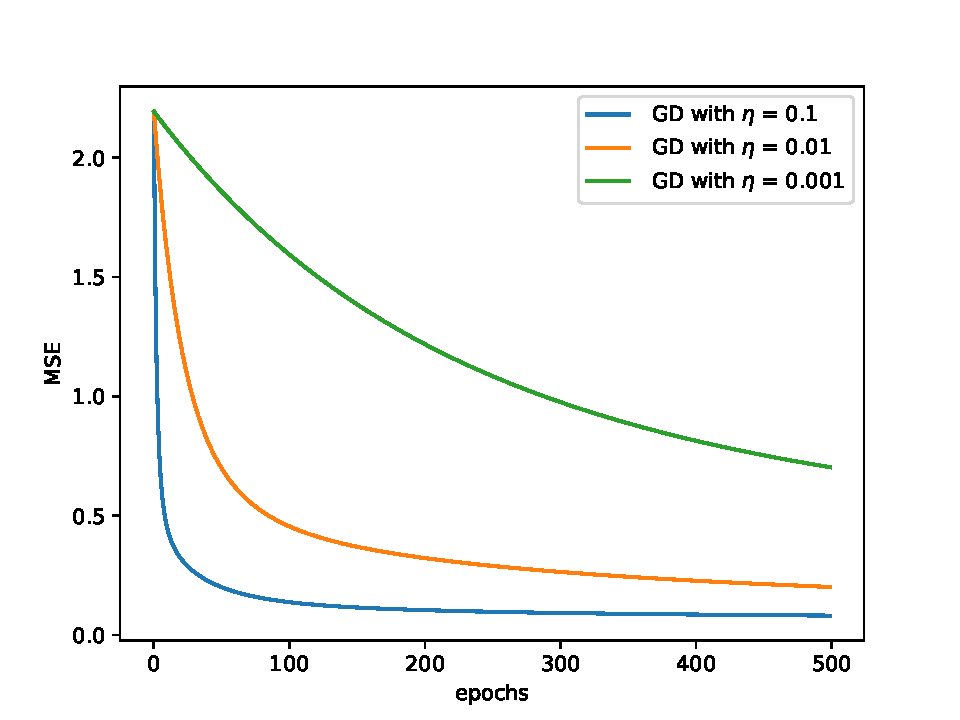
\includegraphics[width=1.0\linewidth]{Project 2/figures/reg/GD_epochs.pdf} 
    \caption{How the MSE for Franke's function varies with epochs for the GD method, for fixed learning rates $\eta=0.1$, $0.01$ and $0.001$. }
    \label{fig: a1}
\end{figure}
This is further supported by figure~\ref{fig: a2}, where we visualize the MSE as a function of both the l2 parameter and the learningrate. The number of epochs is set to 300, and the number of batches is set to 64. The batches and number of operations have been plotted as a colormap where we see the MSE in figure 12
%~\ref{fig: a3}
in the appendix, where we note that the SGD approaches GD when we only have 1 batch. 
%A greater number of batches mean that the convergence rate increases, and we spend less time on each operation. 
From figure~\ref{fig: a2}, we see that we obtain an MSE of 0.06854 for $\eta=0.1$ and the lowest l2 parameter. This is an improvement compared to the MSE obtained for the OLS method and the Ridge method with bootstraps, which we implemented in project 1~\cite{proj1}. 
\begin{figure}[h!]
    \centering %Centers the figure
    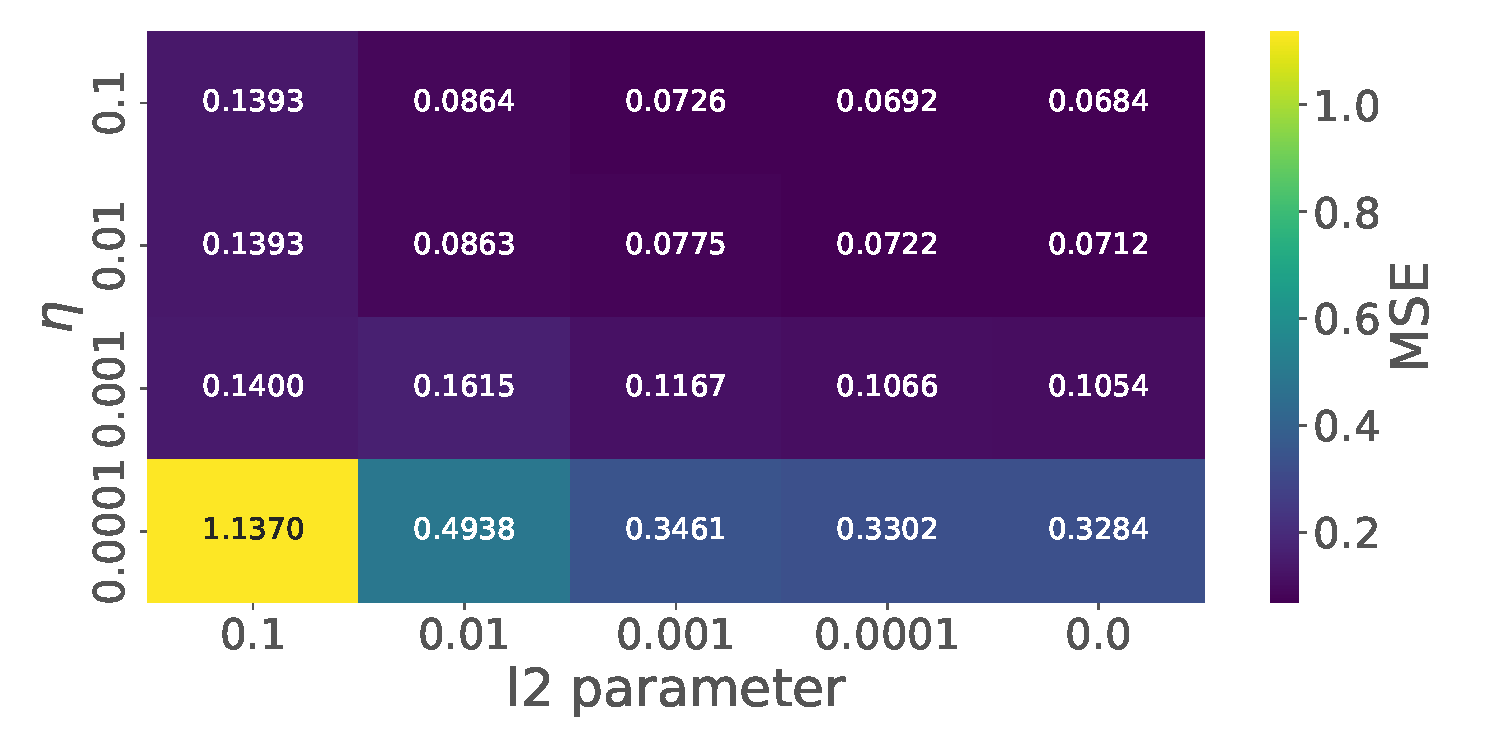
\includegraphics[width=1.0\linewidth]{Project 2/figures/reg/GD_MSE_lambda_eta.pdf} 
    \caption{The MSE for Franke's function for the SGD method as a function of $\eta$ and the l2 parameter, where the number of epochs is 500 and the number of batches is 64.}
    \label{fig: a2}
\end{figure}
\vspace{3mm}
\\ 
We implemented several methods for tuning the learning rate, presented in figure 13
%~\ref{fig: extra1} 
 in appendix~\ref{app: figures}. 
All new methods converge faster than the GD method does, with the RMSprop method being the fastest and most stable method. Both the Adagrad with and without momentum also perform well. 
However, after a certain number of operations the MSE is low for all methods, which can also be seen in table~\ref{table: tab2}. 
\begin{table}[]
\begin{tabular}{|l|ll|}
\hline
\multirow{2}{*}{Method} & \multicolumn{2}{l|}{Time {[}s{]}}                     \\ \cline{2-3} 
                        & \multicolumn{1}{l|}{299 iterations} & 1025 iterations \\ \hline
GD                      & \multicolumn{1}{l|}{0.0922}         & 0.0731          \\ \hline
GD w/ momentum          & \multicolumn{1}{l|}{0.0841}         & 0.0717          \\ \hline
Adagrad                 & \multicolumn{1}{l|}{0.0875}         & 0.0722          \\ \hline
Adagrad w/momentum      & \multicolumn{1}{l|}{0.0796}         & 0.0705          \\ \hline
RMSprop                 & \multicolumn{1}{l|}{0.0710}         & 0.0691          \\ \hline
ADAM                    & \multicolumn{1}{l|}{0.0689}         & 0.0670          \\ \hline
\end{tabular}
\caption{MSE for various methods for two different iterations, for the GD algorithm on the Franke function. After a certain number of operations the MSE is relatively low for all methods. }
\label{table: tab2}
\end{table}
\vspace{3mm}
\\ 
%As we increase the number of batches, the function converges more rapidly, as can be seen in figure~\ref{fig: a2.5}. The convergence rate of SGD approaches the convergence rate of GD as the batch size decreases, and for 1 batch, we have the GD method. 
%\begin{figure}[h!]
%    \centering %Centers the figure
%    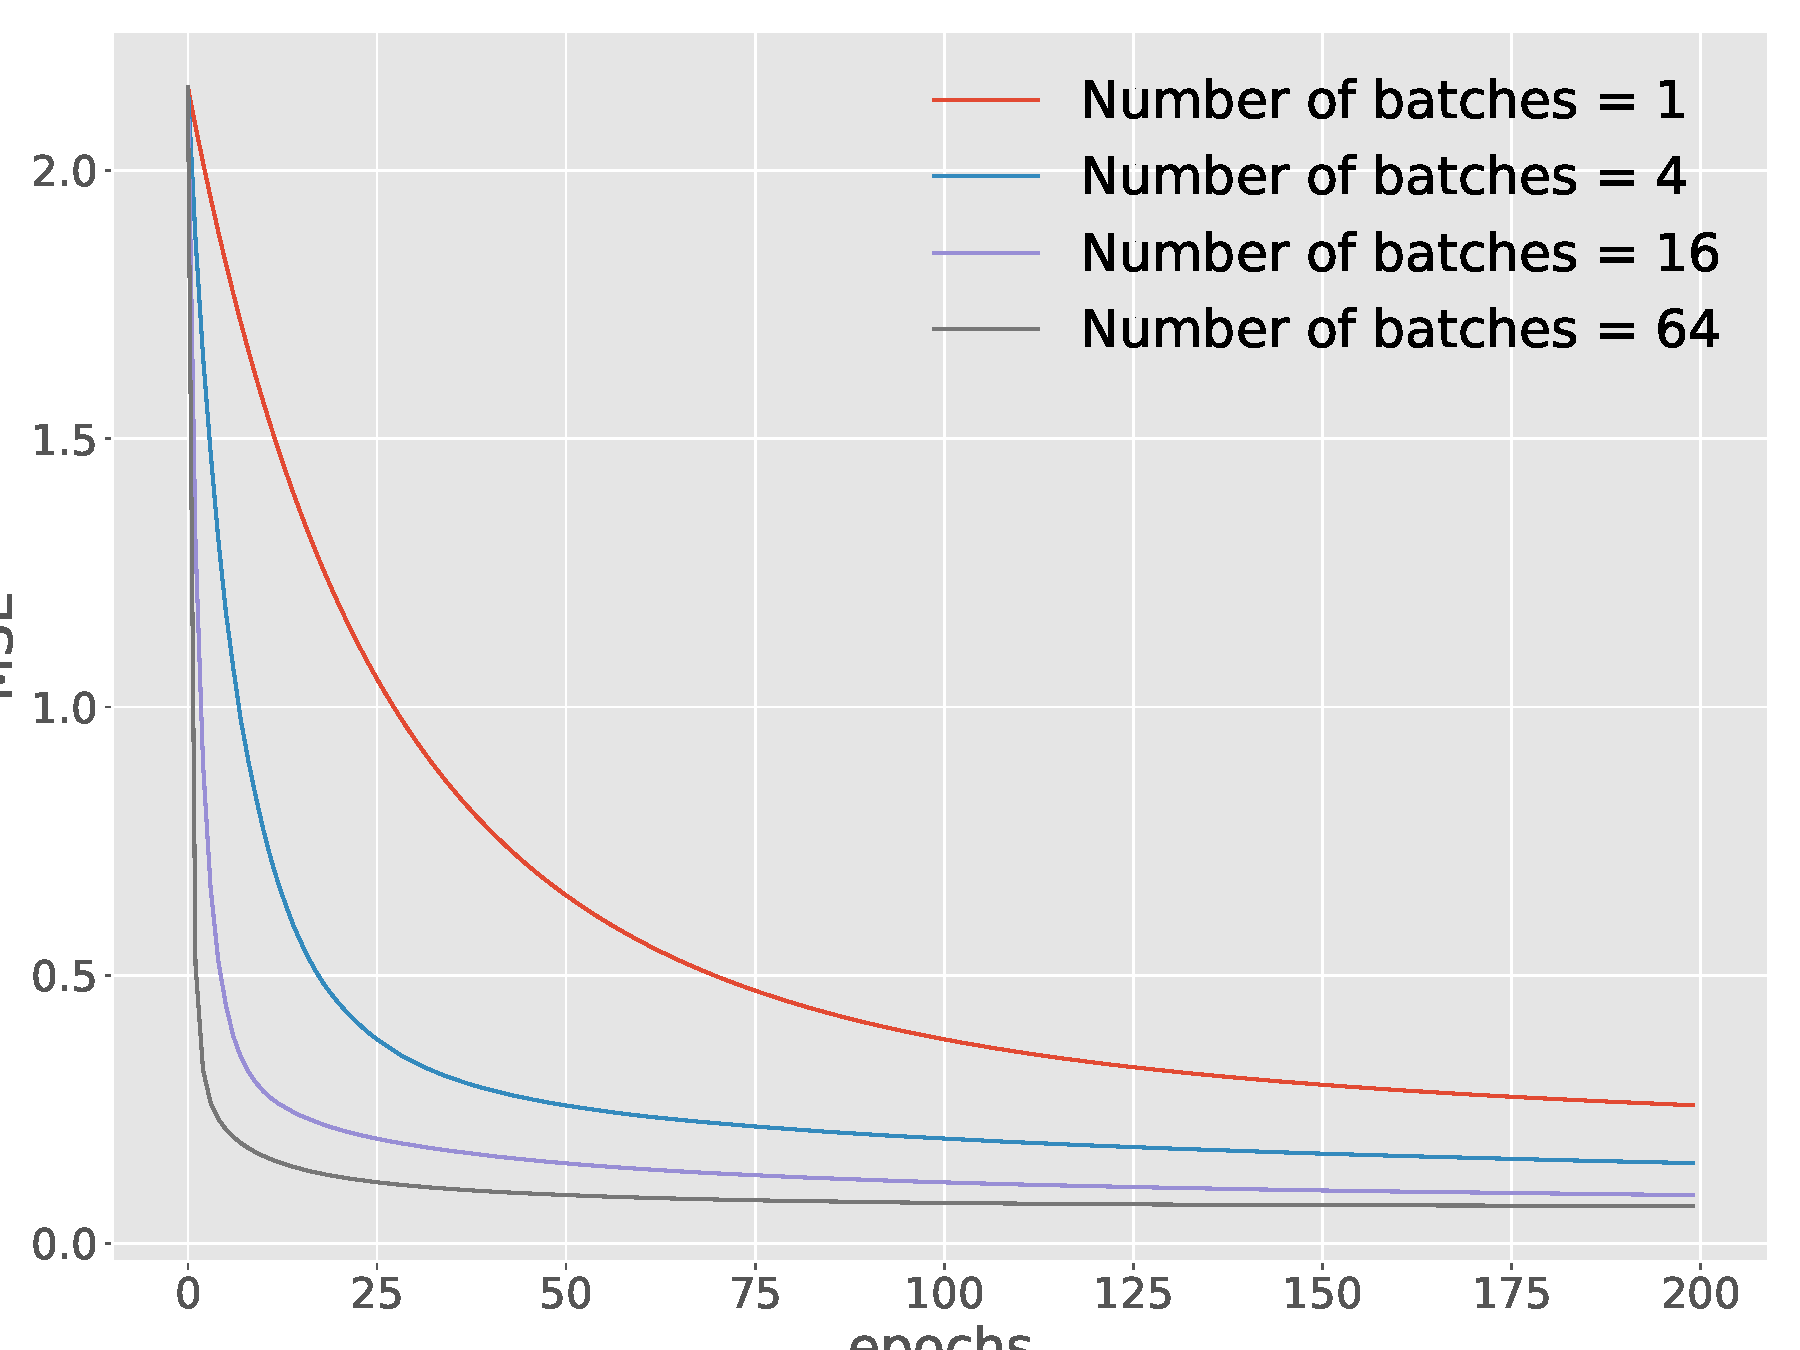
\includegraphics[width=1.0\linewidth]{Project 2/figures/MSE_SG_SGD_batch_sizes.pdf} 
%    \caption{How the MSE for Franke's function varies with epochs for the SGD method, for varying batch sizes, with %a fixed learning rate $\eta=0.01$.}
%    \label{fig: a2.5}
%\end{figure}
%\vspace{3mm}
%\\
In table~\ref{table: a1} we have studied the speed of the GD and SGD in further detail, by calculating the speed per epoch and speed of each operation for $\eta=0.1$ and $\eta=0.01$. While the SGD is slower per epochs, it is much faster per step. 
%as gradients are computed from 5 points at a time, rather than 1000 (N/M) ? 
%If we take the same time, 1000 iterations, 100 epochs * 10 batches 
%We need the number of iterations to be equal to the number of epochs times batches, because if this is the case it will take the same amount of time. 
Due to the randomness of SGD, it is possible for a local minima to be overcome as there is no confinement. Overall, the SGD method seems to overall be an improvement to the GD method, achieving the same MSE as GD in a shorter amount of time. 
\begin{table}[]
\begin{tabular}{|l|ll|ll|}
\hline
\multicolumn{1}{|c|}{\textbf{Method}} & \multicolumn{2}{c|}{GD}     & \multicolumn{2}{c|}{SGD}                       \\ \hline
$\eta$                                & \multicolumn{1}{l|}{0.1}    & 0.01   & \multicolumn{1}{l|}{0.1}     & 0.01   \\ \hline
Time per epochs [ms]                  & \multicolumn{1}{l|}{0.1224} & 0.1097 & \multicolumn{1}{l|}{0.2733}  & 0.2616 \\ \hline
Time per operation [ms]               & \multicolumn{1}{l|}{0.1224} & 0.1097 & \multicolumn{1}{l|}{0.0683}  & 0.0554 \\ \hline
\end{tabular}
\caption{Speed per epochs of GD and SGD, for $\eta=0.1$ and $\eta=0.01$. The number of epochs was set to 500 and the            number of batches to 4. }
\label{table: a1}
\end{table}
\vspace{3mm}
\\ 
% Part b) Writing your own Neural Network code 
We analyze the same regression problem for the Franke function using the FFNN implementation. We begin by using the Sigmoid function as an activation function for the hidden layers, initializing the weights using a normal distribution. 
\vspace{3mm}
\\ 
The method will be affected by the number of hidden layers, nodes, batches, epochs and the learning parameters. We began by analyzing the number of hidden layers and nodes, using the values based on what we found for SGD in the previous analysis for the remaining parameters. The grid search for the optimal MSE depending on hidden layers and nodes is presented in figure 14
%~\ref{fig: b_sigmoid_1}
, in the appendix. 
The best results are obtained for 3 hidden layers and 30 neurons, and we use these values when investigating the choices for the batches and epochs, presented in figure 15
%~\ref{fig: b_sigmoid_2}
in the appendix. Based on this analysis, we see how we need fewer iterations if the number of batches is high enough. Using a high number of batches spends more computational time, but it can also save time for the right number of iterations. Compromising between minimizing the MSE and keeping the computational time satisfactory, we set the batches to 32. 
\vspace{3mm}
\\ 
% Part c) Testing different activation functions 
Now we may perform the grid search for the learning rate $\eta$ and optimization parameter $\lambda$, presented in figure~\ref{fig: b_sigmoid_3}. We see how, for higher values for the learning parameter, the accuracy increases. However, for too high values of $\eta$ we see that no convergence happens, represented by the gray areas. Similar to what we saw for the logistic regression analysis, the optimization parameter has the lowest MSE for $\lambda = 0.00001$, and the lowest MSE overall is where $\eta=0.1$. 
\begin{figure}[h!]
    \centering %Centers the figure
    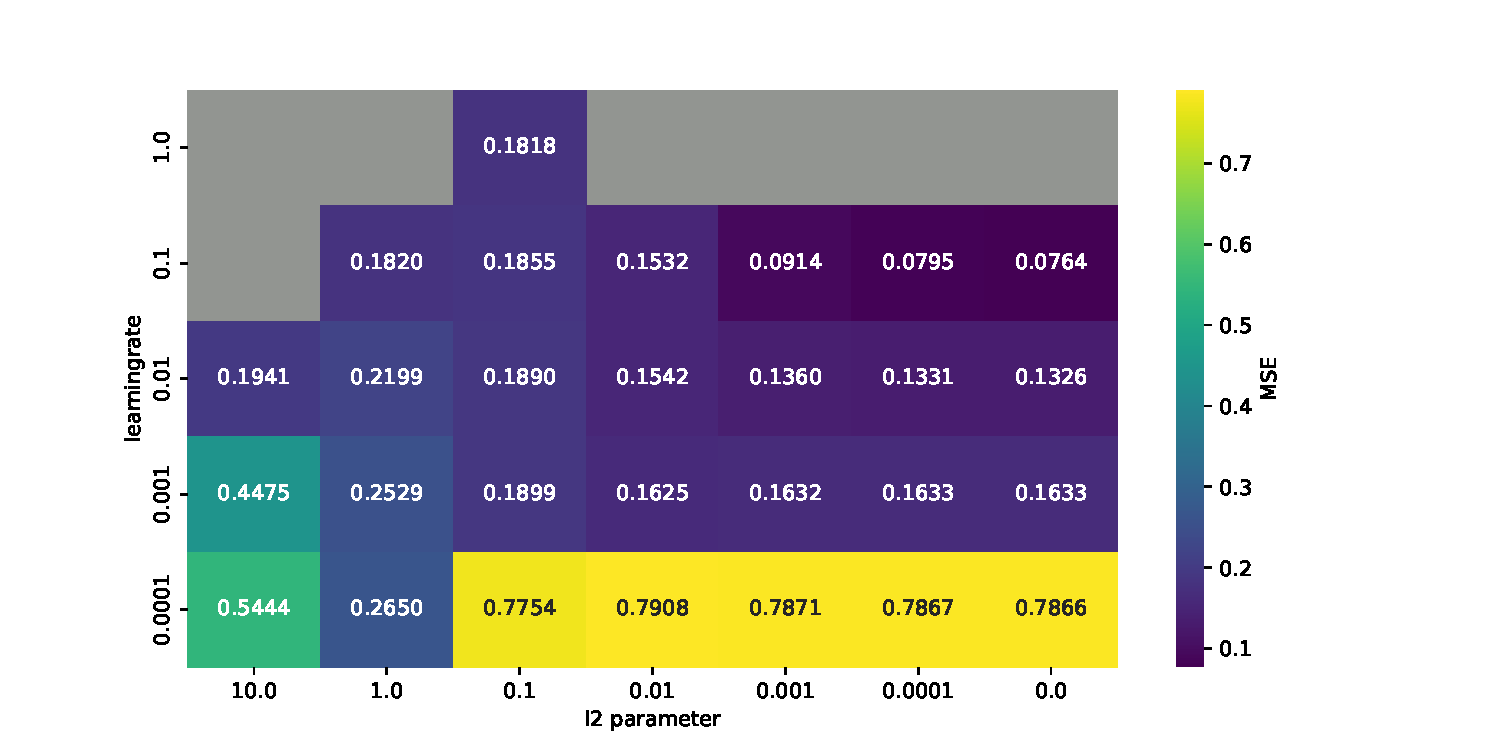
\includegraphics[width=1.0\linewidth]{Project 2/figures/reg/NN_reg_sigmoid_l2_eta.pdf} 
    \caption{How the MSE for Franke's function varies with $\eta$ and $\lambda$, using the Sigmoid function as an activation function. 
    Hidden layers = 3, Neurons = 30, number of batches = 32, epochs = 300.}
    \label{fig: b_sigmoid_3}
\end{figure}
\begin{figure}[h!]
    \centering %Centers the figure
    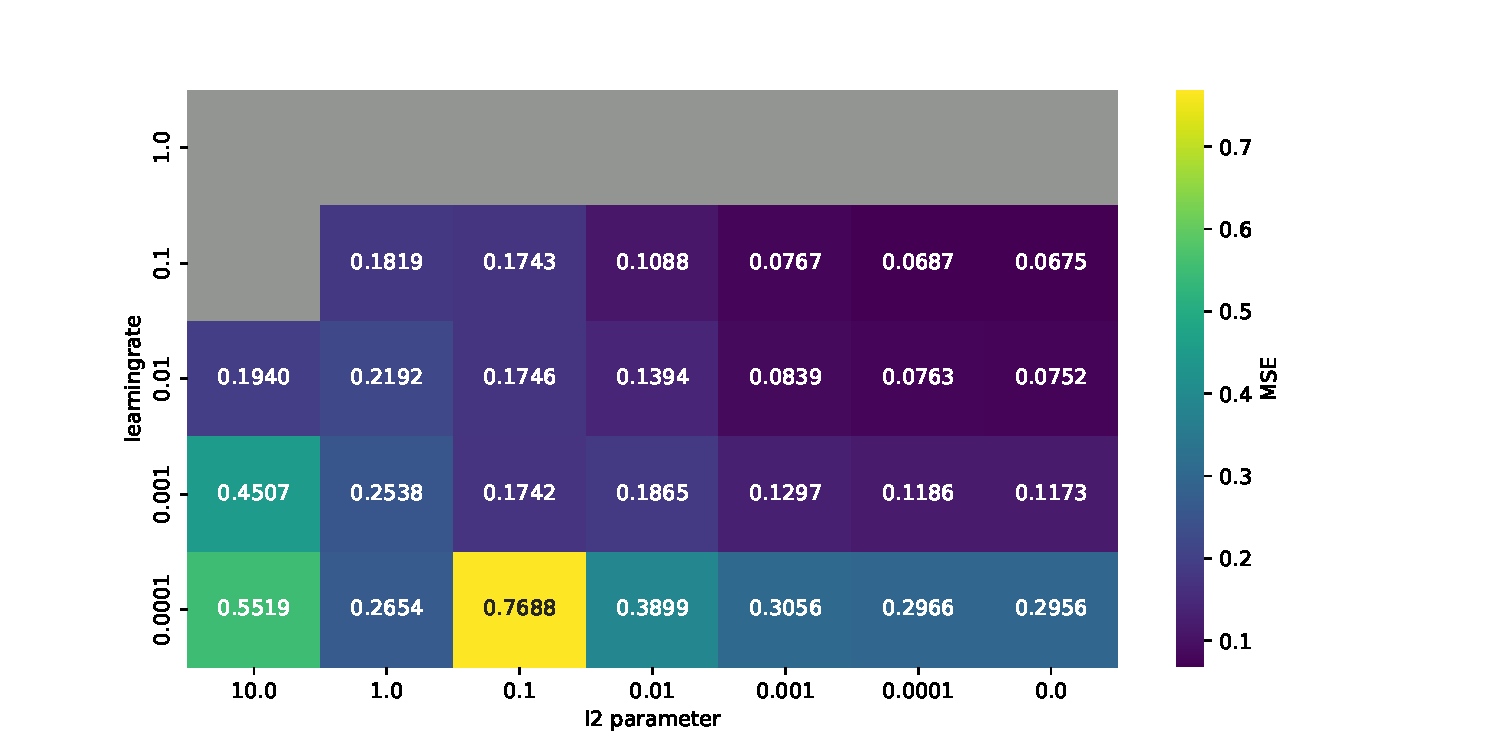
\includegraphics[width=1.0\linewidth]{Project 2/figures/reg/NN_reg_relu_l2_eta.pdf} 
    \caption{How the MSE for Franke's function varies with $\eta$ and $\lambda$, using the ReLu as an activation function. 
    Hidden layers = 3, Neurons = 30, number of batches = 32, epochs = 300.}
    \label{fig: b_relu}
\end{figure}
\begin{figure}[h!]
    \centering %Centers the figure
    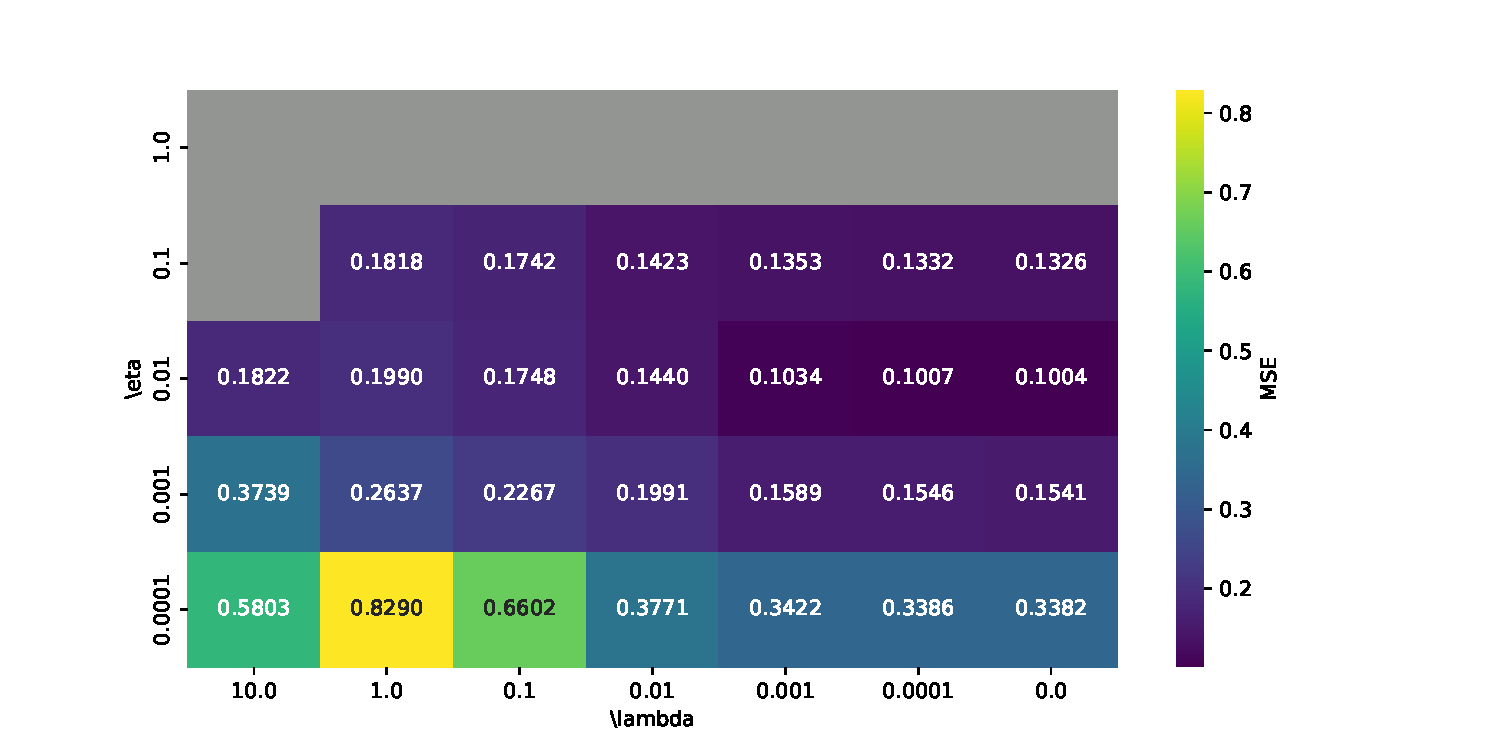
\includegraphics[width=1.0\linewidth]{Project 2/figures/reg/NN_reg_leaky_relu_l2_eta.pdf} 
    \caption{How the MSE for Franke's function varies with $\eta$ and $\lambda$, using the Leaky ReLu as an activation function. 
    Hidden layers = 3, Neurons = 30, number of batches = 32, epochs = 300.}
    \label{fig: b_lrelu}
\end{figure}
Next, we test how different activation functions affect these results, for the same parameters. 
We do not see any improvement for the MSE when using the ReLu as an activation function, seen in figure~\ref{fig: b_relu}, and the Leaky ReLu activation function is significantly worse in this case, seen in figure~\ref{fig: b_lrelu}. 
The lowest MSE=0.0675 is obtained when using Sigmoid. This is quite an improvement compared to the Ridge regression code from the previous project where we had an MSE around 0.1200 when using bootstrapping as the resampling tehnique. However, when we used cross-validation as the resampling technique, we got a lower MSE for Ridge, around 0.0112. 
Generally, both the SGD and NN presented here give a lower MSE than the OLS and Ridge regression codes when not using cross validation~\cite{proj1}. 
%\vspace{3mm}
%\\ 
%Im not sure what this is? 
%\begin{figure}[h!]
%    \centering %Centers the figure
%    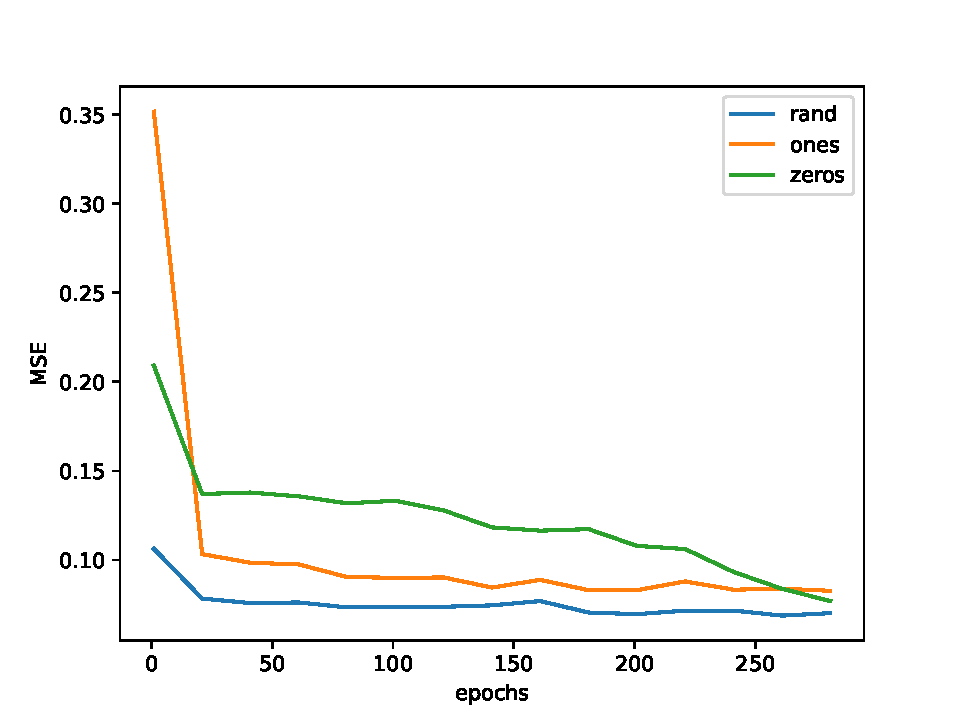
\includegraphics[width=1.0\linewidth]{Project 2/figures/reg/NN_reg_bias.pdf} 
%    \caption{How the MSE for Franke's funciton varies with epochs, depending on the initialized bias. A random initialization gives a better result.}
%    \label{fig: b_bias}
%\end{figure}





\subsection*{Classification Analysis}%__________________________________________________________________
% Part d) Classification analysis using neural networks 
When we study the Wisconsin Breast Cancer data set, we change the cost function for the neural network code in order to perform a classification analysis. The performance is measured with the accuracy score. 
\vspace{3mm}
\\ 
We begin by finding suitable parameters for the number of hidden layers and neurons, seen in the heatmap in figure 16
%~\ref{fig: nn_neuron_layer}
, and then the number of batches and epochs, presented in figure 17
%~\ref{fig: nn_iter_batch}
, both in the appendix. 
The resulting lowest MSE for the neural network code is 0.9825, for $\eta$ = 0.1 and an l2 parameter of 0.00001. 

\begin{figure}[h!]
    \centering %Centers the figure
    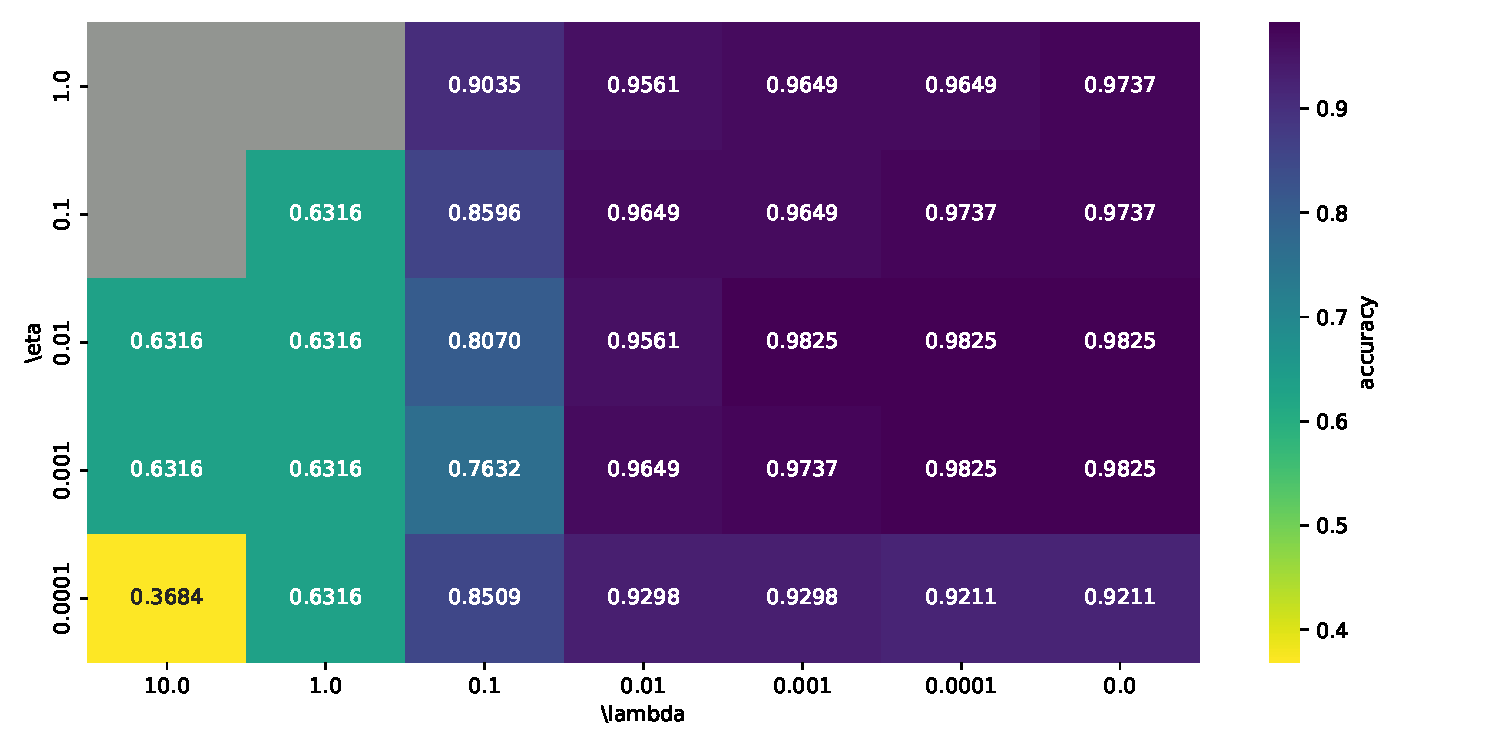
\includegraphics[width=1.0\linewidth]{Project 2/figures/class/NN_class_sigmoid_l2_eta.pdf} 
    \caption{How the MSE for the Wisconsin Breast Cancer data varies with $\eta$ and $\lambda$, using the Sigmoid function as an activation function. Hidden layers = 1, neurons = 25, number of batches = 64, epochs = 768
    }
    \label{fig: nn_l2_eta}
\end{figure}



% Part e) Logistic Regression code 
Finally, we want to compare the neural network classification results with the results we are able to obtain using another method, in this case the results we obtain from the logistic regression code using the SGD algorithm. 
\vspace{3mm}
\\ 
We begin by looking at the accuracy for SGD for different l2 parameters and different learningrates, comparing the GD algorithm, seen in figure~\ref{fig: gd_lambda_eta} with ADAM seen in figure~\ref{fig: adam_lambda_eta}. The accuracy when using ADAM are somewhat higher than the results with SGD, with a difference of around 0.01 between the highest accuracy scores for both. The best scores with SGD are for a low learningparameter, while the best scores with ADAM are for a slightly higher learningparameter, at $0.0001$. 
\begin{figure}[h!]
    \centering %Centers the figure
    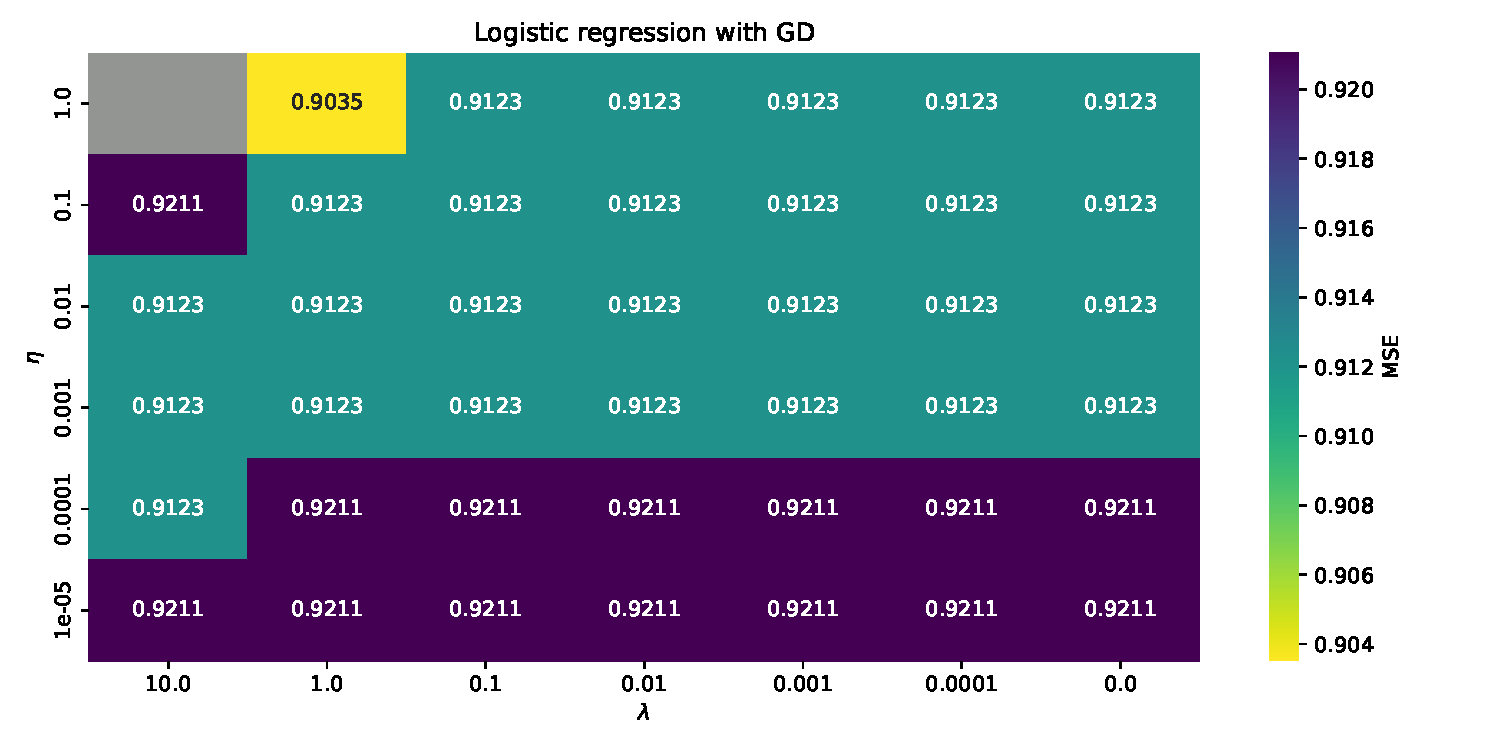
\includegraphics[width=1.0\linewidth]{Project 2/figures/class/GD_acc_lambda_eta.pdf} 
    \caption{Accuracy score for SGD as a function of the learningparameter $\eta$ and the l2 parameter $\lambda$, for epochs = 1024 and batches = 1.}
    \label{fig: gd_lambda_eta}
\end{figure}
\begin{figure}[h!]
    \centering %Centers the figure
    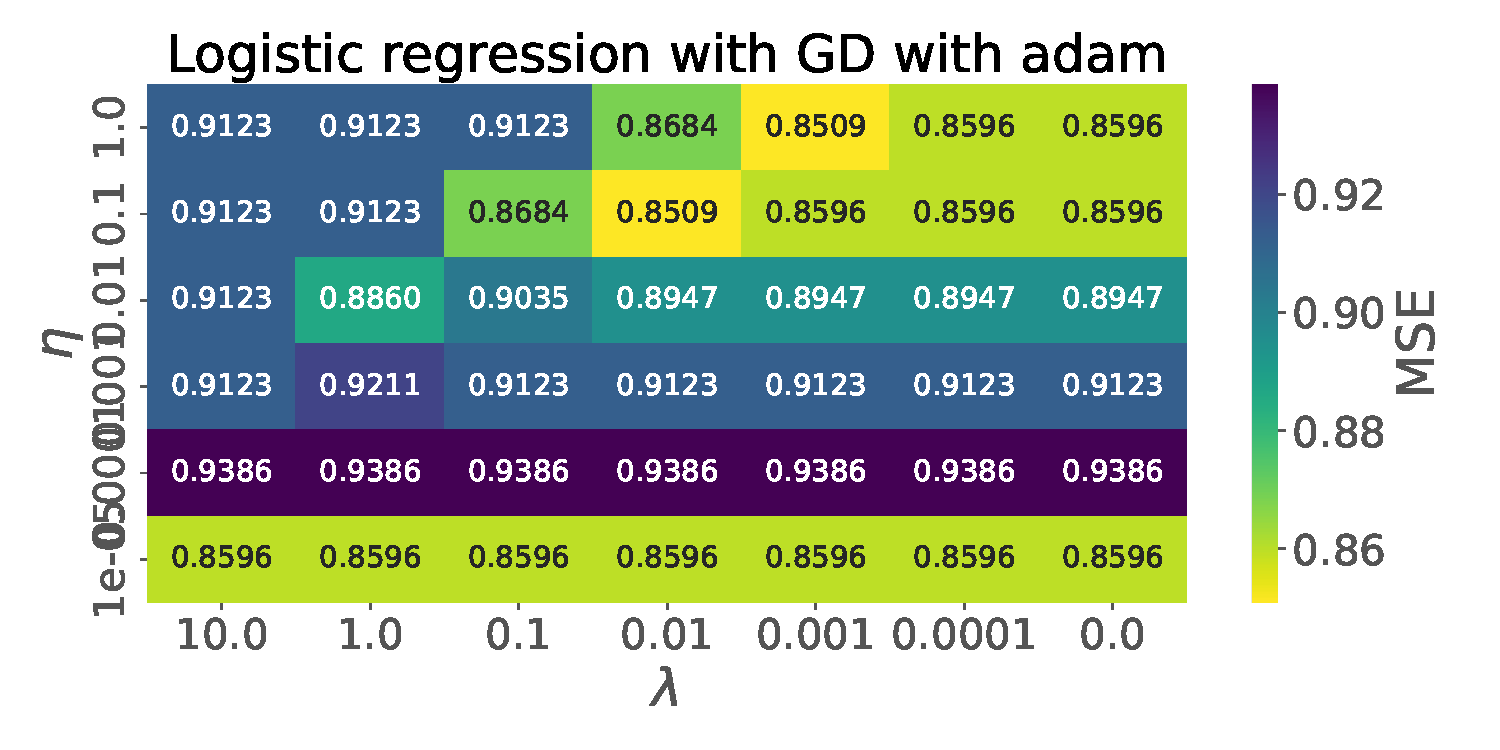
\includegraphics[width=1.0\linewidth]{Project 2/figures/class/adam_acc_lambda_eta.pdf} 
    \caption{Accuracy score for ADAM as a function of the learningparameter $\eta$ and the l2 parameter $\lambda$, for epochs = 1024 and batches = 1.}
    \label{fig: adam_lambda_eta}
\end{figure}
\vspace{3mm}
\\ 
Next, we study the accuracy for SGD with ADAM for a different number of batches and number of operations, seen in figure~\ref{fig: op_batch}. 
\begin{figure}[h!]
    \centering %Centers the figure
    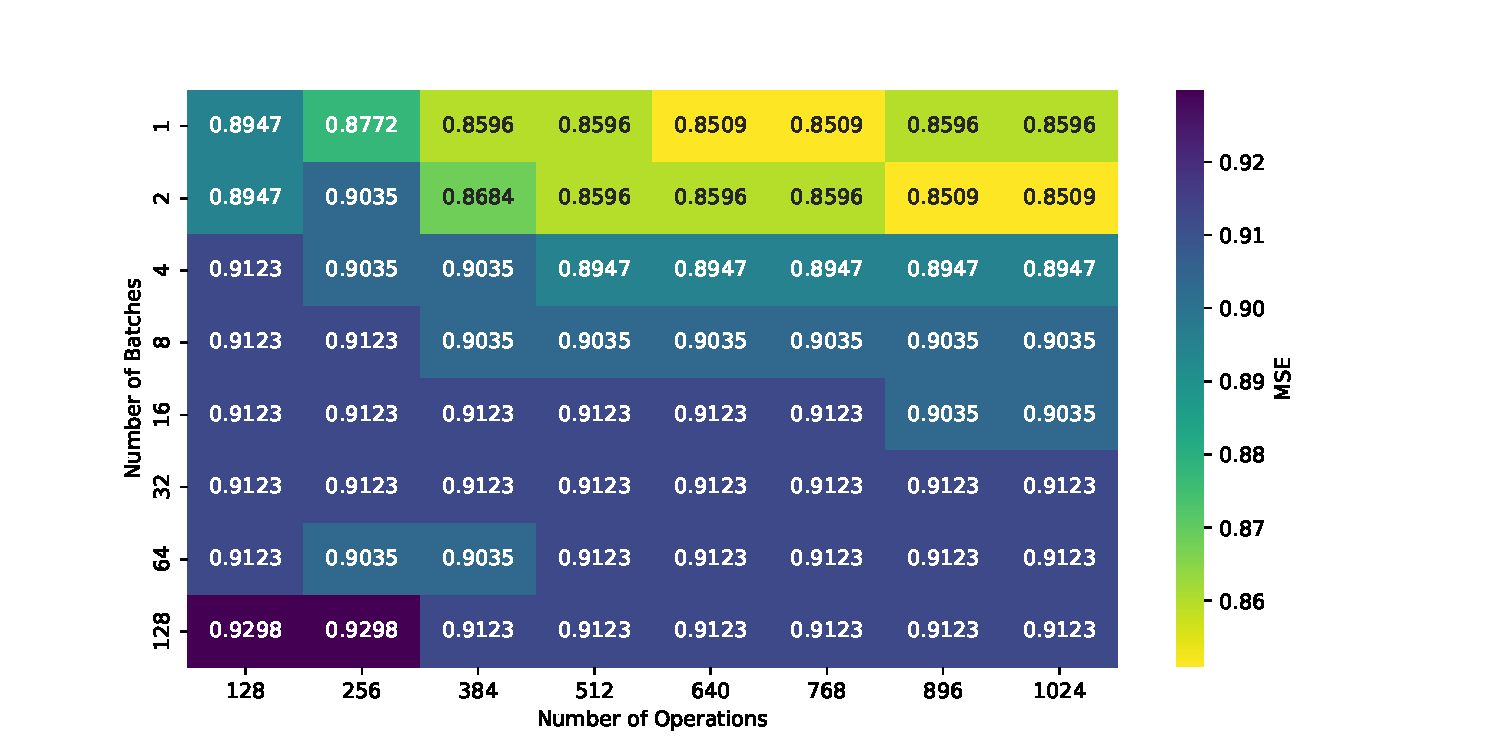
\includegraphics[width=1.0\linewidth]{Project 2/figures/class/SGD_operations_batches_0.1.pdf} 
    \caption{Accuracy score using logistic regression as a function of the number of batches and the number of operations, for epochs = 1024, batches = 1, eta=0.001, and l2=0.0}
    \label{fig: op_batch}
\end{figure}
\vspace{3mm}
\\ 
Finally, we can compare our results with the accuracy we obtain when using scikit learn's logistic regression function, for which we obtain a test set accuracy of 0.9474. This is higher than what we obtained using our own logistic regression code, where we obtain an accuracy of 0.9386 when using ADAM. It is still lower than the score we got for the neural networks code, where we obtained an accuracy score of 0.9825. 
    









%___________________________DISCUSSION___________________________________
%\section{Results and Discussion}\label{sec:discussion}
% Regression analysis for the Franke function 
%___________________________CONCLUSION______________________________________
\section{Conclusion}\label{sec:conclusion}
% Present results and error margin 
In this report we have studied various methods while investigating classification and regression problems. 
We found that while all methods provide us with a descent accuracy, the neural network is better suited for classification problems, where we achieved a higher accuracy score than both our own logistic regression code and the accuracy score obtained from scikit learn's algorithm. Meanwhile, for the regression analysis we saw that surprisingly the Sigmoid function achieved the best results, although by a very small margin compared to the ReLu. The neural network code did not achieve a better accuracy score in this case, however the difference in accuracies between the logistic regression code and the neural network code were lower for the regression problem than it was for the classification problem. 
\vspace{3mm}
\\ 
% We could have obtained even more precise results if we had ...
It is likely that we could have obtained even more precise results if we had spent even more time testing the various parameters, but the results achieved are satisfactory. 
% Further studies may try ...
When studying the regression problem for the Franke function with the FFNN implementation, we have used a fixed number of hidden layers and nodes. Therefore, we are limited by the layers and nodes we set based on the grid search where we search for the best combination of these two parameters. As the parameters are selected based on values for the number of batches, epochs, and learning parameter that might not be the most optimal for the model, this somewhat limits the accuracy of the analysis, and it is possible that even better paramaters could be found for the FFNN implementation. While the MSE values were satisfactory and the models can still be considered accurate, further studies could attempt to implement these in a manner that allows us to study the effect of every parameter in further detail. 
% All in all ... 

%^ acknowledgements (optional)
%\begin{acknowledgments} 
%I would like thank myself for writing this beautiful document.
%\end{acknowledgments}

% _________________________________REFERENCES______________________________________
\newpage 
\section*{References}
\printbibliography[heading=none]

\appendix
\section{Algorithms}\label{app: algos}
\subsubsection*{Adagrad} %_______________________________________________________________
The AdaGrad algorithm adaptively scales the learning rate for each dimension. We implement it by iterating over the epochs, and then for every epoch we iterate through the mini-batches, as explained in algorithm~\ref{algo: Adagrad}. %Batches are random intervals. 

% Algorithm for Adagrad
\begin{algorithm}[H]
    \caption{Adagrad}\label{algo: Adagrad}
    \begin{algorithmic}
        \While{in epochs} \Comment{Iterate through epochs}
        \While{in mini-batches} \Comment{Iterate through the}%\Comment{Batches are random intervals}
        \State $\:\:\:\:\:\:\:\:\:\:\:\:\:\:\:\:\:\:\:\:\:\:\:\:\:\:\:\:\:\:\:\:\:\:\:\:\:\:\:\:\:\:\:\:\:\:\:\:\:\:\:\:\:\:\:\:\:\:\:\:\:\:\:\:\:\:\:\:\:\:\:\:\:\:\:\:\:\:\:\:$ mini-batches
        \State $\mathbf{g}_t \leftarrow \nabla_\theta \mathcal{C}(\boldsymbol{\theta})$ 
        \State $\theta_{t+1} \leftarrow \mathbf{g}_t \eta \frac{1}{\sqrt{\delta+ \sum^t(\mathbf{g}_t)^2}}$
    \end{algorithmic}
\end{algorithm}

\subsubsection*{Root Mean Squared Propagation}
RMSprop provides an exponentially decaying average rather than the sum of the gradients. The decaying average is realized by combining the momentum algorithm and the Adagrad algorithm with a new term. The RMSprop method is restricted to the sum of the past gradients, in addition to the gradients for the recent time steps, meaning that it changes the learning rate slowly while converging relatively fast~\cite{lecture_notes}. 

% Algorithm for RMSprop
\begin{algorithm}[H]
    \caption{RMSprop}\label{algo: RMSprop}
    \begin{algorithmic}
        \While{in epochs} \Comment{Iterate through epochs}
        \State $k \leftarrow 0$
        \While{in mini-batches} \Comment{Iterate through the}%\Comment{Batches are random intervals}
        \State $\:\:\:\:\:\:\:\:\:\:\:\:\:\:\:\:\:\:\:\:\:\:\:\:\:\:\:\:\:\:\:\:\:\:\:\:\:\:\:\:\:\:\:\:\:\:\:\:\:\:\:\:\:\:\:\:\:\:\:\:\:\:\:\:\:\:\:\:\:\:\:\:\:\:\:\:\:\:\:\:$ mini-batches
        \State $\mathbf{g}_t \leftarrow \nabla_\theta \mathcal{C}(\boldsymbol{\theta})$
        \State $k \leftarrow (\rho k + (1 - \rho)\mathbf{g}_t \mathbf{g}_t)$
        \Comment{Scaling with $\rho$}
        \State $\theta_{t+1} \leftarrow \mathbf{g}_t \eta \frac{1}{\sqrt{\delta + k}}$
        \Comment{Inverting the diagonal}
    \end{algorithmic}
\end{algorithm}

\subsubsection*{Adam} %_______________________________________________________________
Another related algorithm is the Adam optimizer, which is efficient when working with large problems involving a lot of data and parameters. 
The algorithm~\ref{algo: ADAM} keeps a running average of both the first and second moment of the gradient and uses this information to adaptively change the learning rate for different parameters. 

% Algorithm for ADAM 
\begin{algorithm}[H]
    \caption{ADAM}\label{algo: ADAM}
    \begin{algorithmic}
        \State m_0 \leftarrow 0.0 \Comment{Initialize first moment}
        \State s_0 \leftarrow 0.0 \Comment{Initialize second moment}
        \While{in epochs} \Comment{Iterate through epochs}
        \While{in mini-batches} \Comment{Iterate through the}%\Comment{Batches are random intervals}
        \State $\:\:\:\:\:\:\:\:\:\:\:\:\:\:\:\:\:\:\:\:\:\:\:\:\:\:\:\:\:\:\:\:\:\:\:\:\:\:\:\:\:\:\:\:\:\:\:\:\:\:\:\:\:\:\:\:\:\:\:\:\:\:\:\:\:\:\:\:\:\:\:\:\:\:\:\:\:\:\:\:$ mini-batches
        %\State $t \leftarrow t + 1$
        \State $\mathbf{g}_t \leftarrow \nabla_\theta \mathcal{C}(\boldsymbol{\theta_})$
        \Comment{Get gradients}
        \State $\mathbf{m}_t \leftarrow \beta_1 \mathbf{m}_{t-1} + (1-\beta_1) \mathbf{g}_t$
        \Comment{Update biased 1st}
        \State $\:\:\:\:\:\:\:\:\:\:\:\:\:\:\:\:\:\:\:\:\:\:\:\:\:\:\:\:\:\:\:\:\:\:\:\:\:\:\:\:\:\:\:\:\:\:\:\:\:\:\:\:\:\:\:\:\:\:\:\:\:\:\:\:\:\:\:\:\:\:\:\:\:\:\:\:\:\:\:\:\:\:\:\:\:\:\:\:\:$ moment
        \State $\boldsymbol{\mathbf{\hat{m}}}_t \leftarrow {\mathbf{m}_t \over 1-\beta_1^t}$
        \Comment{Compute bias-corrected 1st}
        \State $\:\:\:\:\:\:\:\:\:\:\:\:\:\:\:\:\:\:\:\:\:\:\:\:\:\:\:\:\:\:\:\:\:\:\:\:\:\:\:\:\:\:\:\:\:\:\:\:\:\:\:\:\:\:\:\:\:\:\:\:\:\:\:\:\:\:\:\:\:\:\:\:\:\:\:\:\:\:\:\:\:\:\:\:\:\:\:\:\:$ moment
        \State $\mathbf{s}_t \leftarrow \beta_2 \mathbf{s}_{t-1} +(1-\beta_2)\mathbf{g}_t^2$ 
        \Comment{Update biased 2nd}
        \State $\:\:\:\:\:\:\:\:\:\:\:\:\:\:\:\:\:\:\:\:\:\:\:\:\:\:\:\:\:\:\:\:\:\:\:\:\:\:\:\:\:\:\:\:\:\:\:\:\:\:\:\:\:\:\:\:\:\:\:\:\:\:\:\:\:\:\:\:\:\:\:\:\:\:\:\:\:\:\:\:\:\:\:\:\:\:\:\:\:$ moment
        \State $\boldsymbol{\mathbf{\hat{s}}}_t \leftarrow {\mathbf{s}_t \over1-\beta_2^t}$
        \Comment{Compute bias-corrected 2nd}
        \State $\:\:\:\:\:\:\:\:\:\:\:\:\:\:\:\:\:\:\:\:\:\:\:\:\:\:\:\:\:\:\:\:\:\:\:\:\:\:\:\:\:\:\:\:\:\:\:\:\:\:\:\:\:\:\:\:\:\:\:\:\:\:\:\:\:\:\:\:\:\:\:\:\:\:\:\:\:\:\:\:\:\:\:\:\:\:\:\:\:$ moment
        \State $\boldsymbol{\theta}_{t+1} \leftarrow \boldsymbol{\theta}_t - \eta_t {         \boldsymbol{\mathbf{m}}_t \over \sqrt{\boldsymbol{\mathbf{s}}_t} +\epsilon}$
        \Comment{Update parameters}
    \end{algorithmic}
\end{algorithm}
The parameters $\beta_1$ and $\beta_2$ set the memory lifetime of the first and second moment and are typically taken to be $0.9$ and $0.99$ respectively, and $\eta$ is the learning rate typically chosen as $10^{-3}$, and $\epsilon$ is a small regularization constant to prevent divergences. 




\section{Back Propagation} %_________________________________________________

Train data based on the cost function (compare network output with training data) 
minimize the cost output (method of adjusting weights and biases by estimating the gradient of the cost function, back propagation) 

f is the activation function 
f'(zj) is the derivative for activation z 
j is node 
k is class or entry 
L is layer 
w and b are the weights and biases 

weight and biase in teh network are typically initialized randomly -> highly unlikely to find good predictions 
Need to iteratively adjust the weights and biases until the predictions are satisfactory 
Called training: We use gradient methods to find the minimum of the models cost functions. Now need to compute the gradients of the cost function with respect to all the weights and biases in the network, which has potentially many weights and biases all dependent on one another, and can become coputationaly heavy 
We therefore make use of the algorithm backpropagation 

Initializing the weights and biases. to get fat covergence or non convergence of the gradient method. Initialize the biases to some small value eprioon (can experiment to find it) and the weights with iniform distribution between -1 and 1 . 

The four equations provide us with a way of computing the gradient of the cost function, for which the method we use is presented in the algorithm~\ref{algo:FFNN_BP} for back propagation, where the parameter $\eta$ is the learning parameter discussed in connection with the gradient descent methods. 
XXX: Here it is convenient to use stochastic gradient descent (see the examples below) with mini-batches with an outer loop that steps through multiple epochs of training. 

% Algorithm for Back propagation
\begin{algorithm}[H]
    \caption{Back Propagation}\label{algo:FFNN_BP}
    \begin{algorithmic}
        \State XXX 
        \Comment{Set up the input data $\hat{x}$ and the activations $\hat{z}_1$ of the input layer and compute the activation function and the pertinent outputs $\hat{a}^1$} 
        \State XXX
        \Comment{Perform the feed forward until we reach the output layer. Compute all $\hat{z}_l$ of the input layer and the activation function and the pertinent outputs $\hat{a}^l$ for $l=1,2,3,...,L$.}
        \State $\eta = XXX$ \Comment{Initialize the learning rate}
        \State $\delta_j^L \leftarrow f'(z_j^L) \frac{\partial\mathcal{C}}{\partial(a_j^L)}$
        \Comment{Compute the output error $\delta^L$}
        \State $\delta_j^l \leftarrow \sum_k \delta_k^{l+1} w_{kj}^{l+1} f'(z_j^l)$
        \Comment{Compute the back propagate error for each $l = L-1, L-1, ..., 2$}
        \State $w^l_{jk} \leftarrow w^l_{jk} - \eta\delta^l_j a^{l-1}_k$, 
        \Comment{Update the weights and the biases using gradient descent}
        \State $b^l_{j} \leftarrow b^l_{j} - \eta\frac{\partial\mathcal{C}}{\partial b^l_j = b^l_j - \eta\delta^l_j}$
        
    \end{algorithmic}
\end{algorithm}
\vspace{3mm}
\\
When all weights and biases throughout the network have been updated a number epoch times, the cost function preferably decreases. 

The lambda is to prevent overfitting. 
Preventing overditting. Introduce a regularization term (lambda) 






\section{Additional Figures}

\begin{itemize}
\color{white}
\item First item
\item Second item
\end{itemize}

\begin{figure}[h!]
    \centering %Centers the figure
    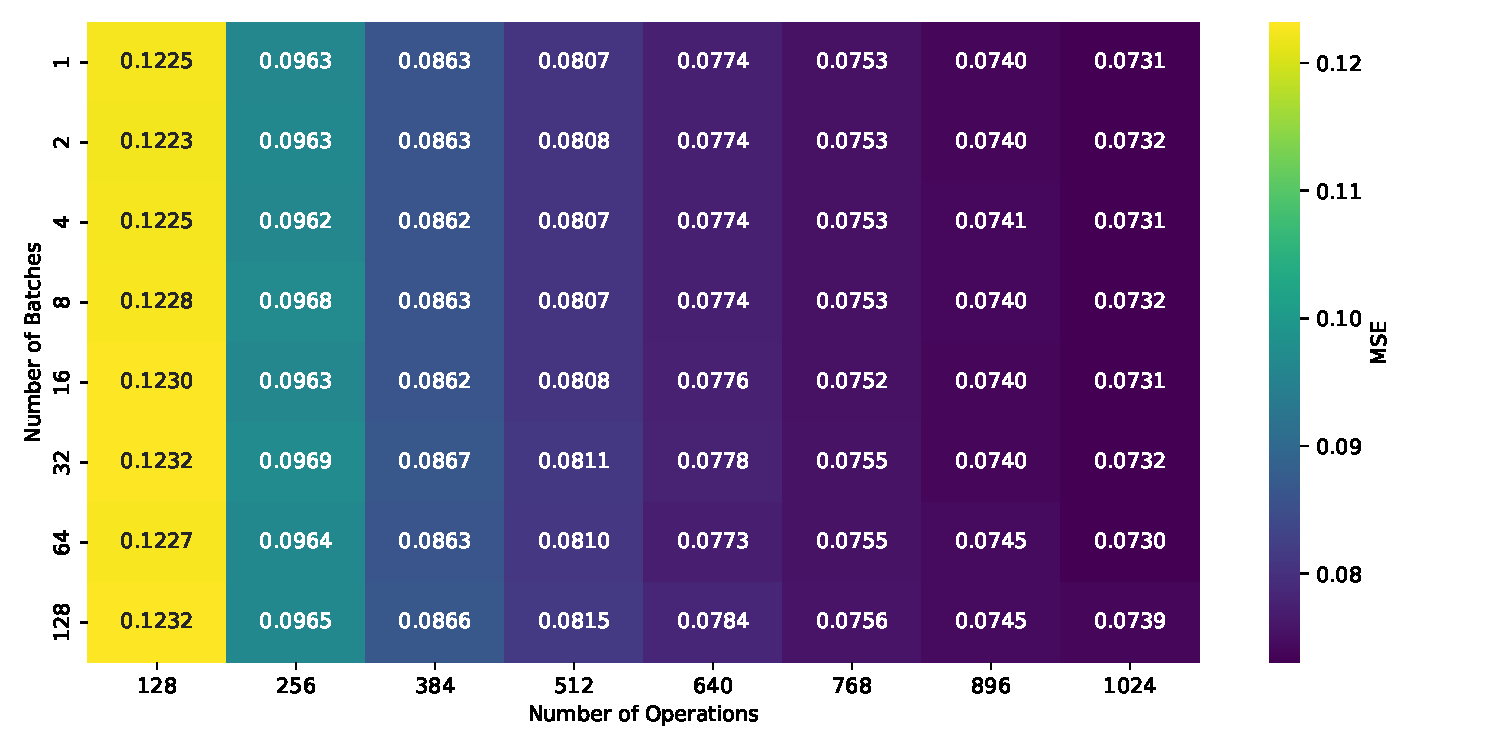
\includegraphics[width=1.0\linewidth]{Project 2/figures/reg/SGD_op_batch.pdf} 
    \caption{How the MSE for Franke's function varies with the batch size and number of operations, for $\eta=0.1$. }
    \label{fig: a3}
\end{figure}

\begin{itemize}
\color{white}
\item First item
\item Second item
\end{itemize}

\begin{figure}[h!]
    \centering %Centers the figure
    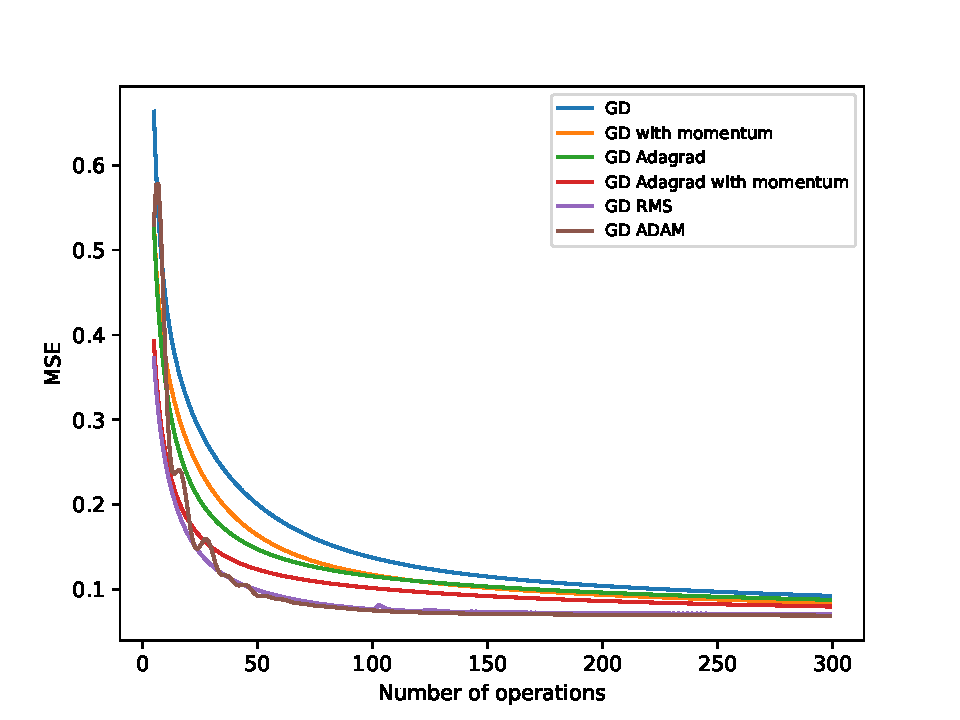
\includegraphics[width=1.0\linewidth]{Project 2/figures/reg/GD_MSE_learningrates_extra.pdf} 
    \caption{How the MSE for Franke's function varies with epochs for the GD method, for $\eta=0.01$.}
    \label{fig: extra1}
\end{figure}

\begin{itemize}
\color{white}
\item First item
\item Second item
\end{itemize}

\begin{figure}[h!]
    \centering %Centers the figure
    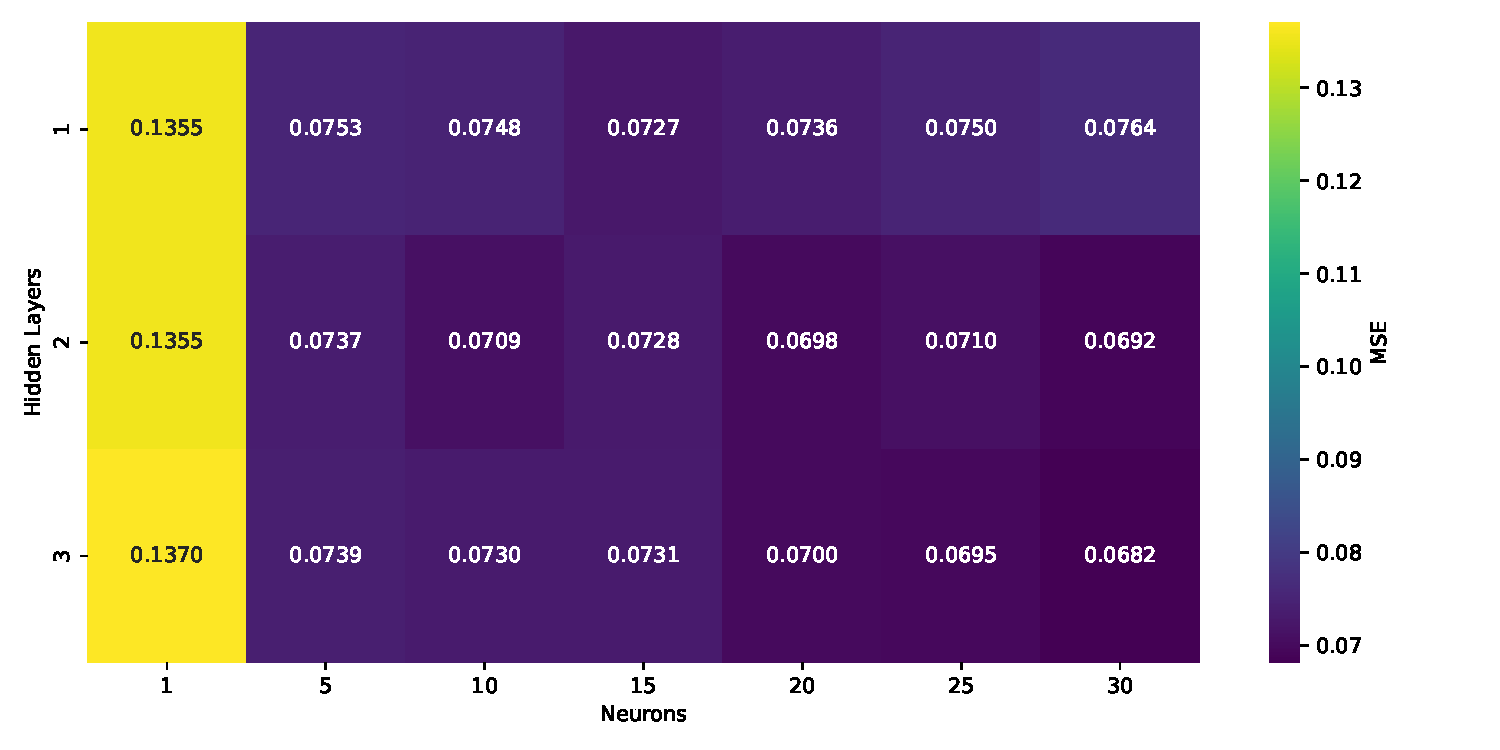
\includegraphics[width=1.0\linewidth]{Project 2/figures/reg/NN_reg_sigmoid_neurons_layers.pdf} 
    \caption{How the MSE for Franke's function varies with the number of hidden layers and neurons, using the Sigmoid function as an activation function. 
    Number of batches = 64, epochs = 300,  $\eta=0.1$.
    }
    \label{fig: b_sigmoid_1}
\end{figure}

\begin{itemize}
\color{white}
\item First item
\item Second item
\end{itemize}

\begin{figure}[h!]
    \centering %Centers the figure
    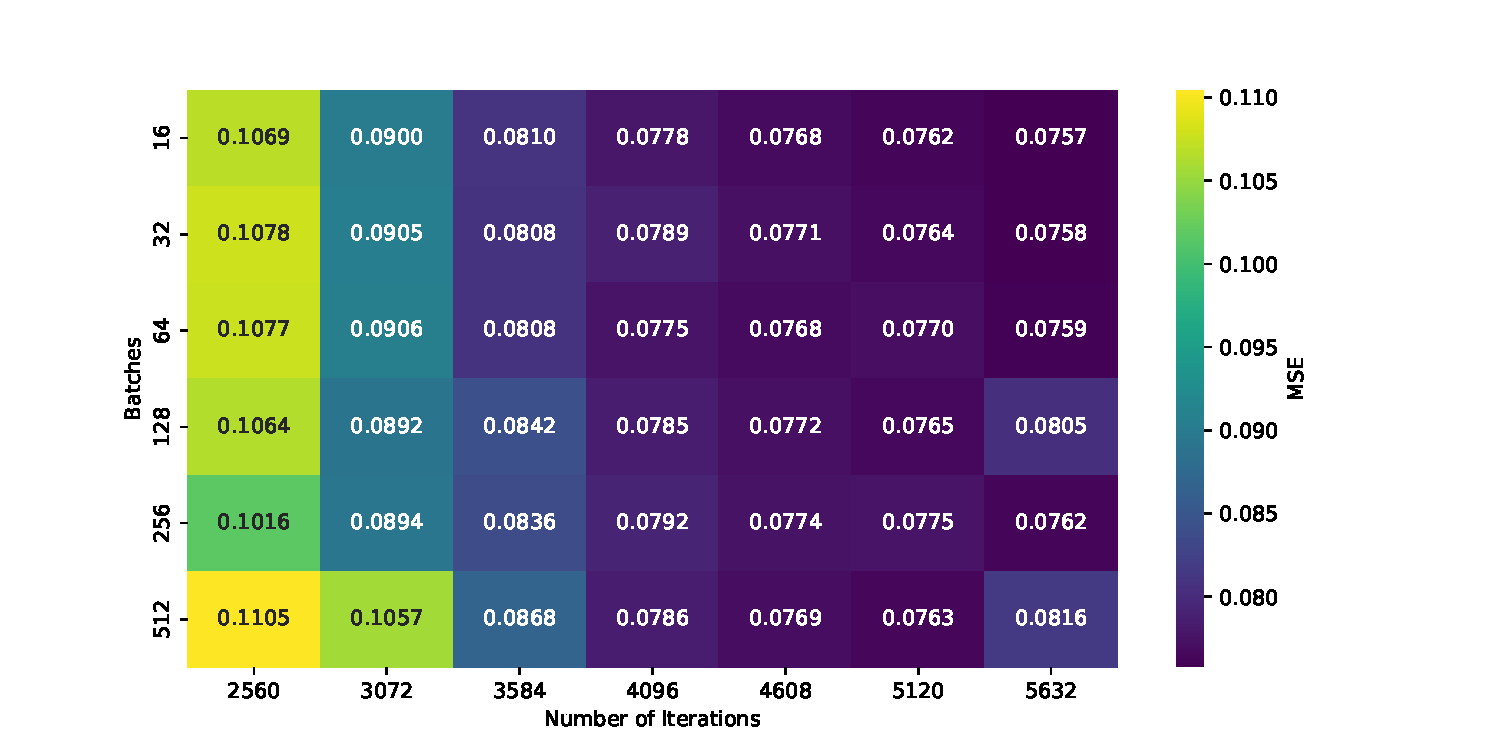
\includegraphics[width=1.0\linewidth]{Project 2/figures/reg/NN_reg_sigmoid_iterations_batches.pdf} 
    \caption{How the MSE for Franke's function varies with the batches and epochs, using the Sigmoid function as an activation function. 
    Hidden layers = 3, Neurons = 30, $\eta=0.1$, and l2 = 0.00001}
    \label{fig: b_sigmoid_2}
\end{figure}


\begin{itemize}
\color{white}
\item First item
\item Second item
\end{itemize}


\begin{figure}[h!]
    \centering %Centers the figure
    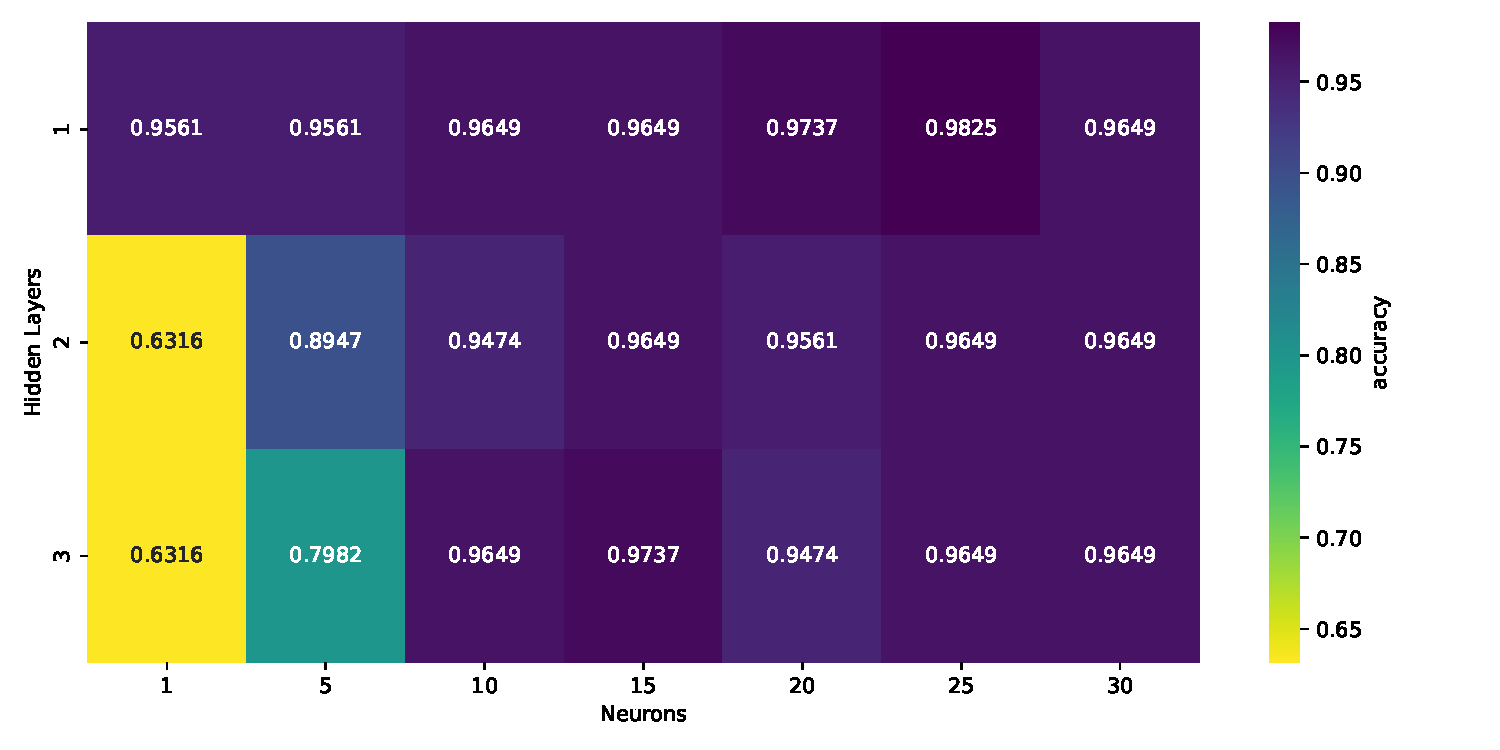
\includegraphics[width=1.0\linewidth]{Project 2/figures/class/NN_class_sigmoid_neurons_layers.pdf} 
    \caption{How the MSE for the MSE for the Wisconsin Breast Cancer data varies with the batches and epochs, using the Sigmoid function as an activation function. Batches = 1, epochs = 640, $\eta$ = 0.1, l2=0.0
    }
    \label{fig: nn_neuron_layer}
\end{figure}


\begin{itemize}
\color{white}
\item First item
\item Second item
\end{itemize}

\begin{figure}[h!]
    \centering %Centers the figure
    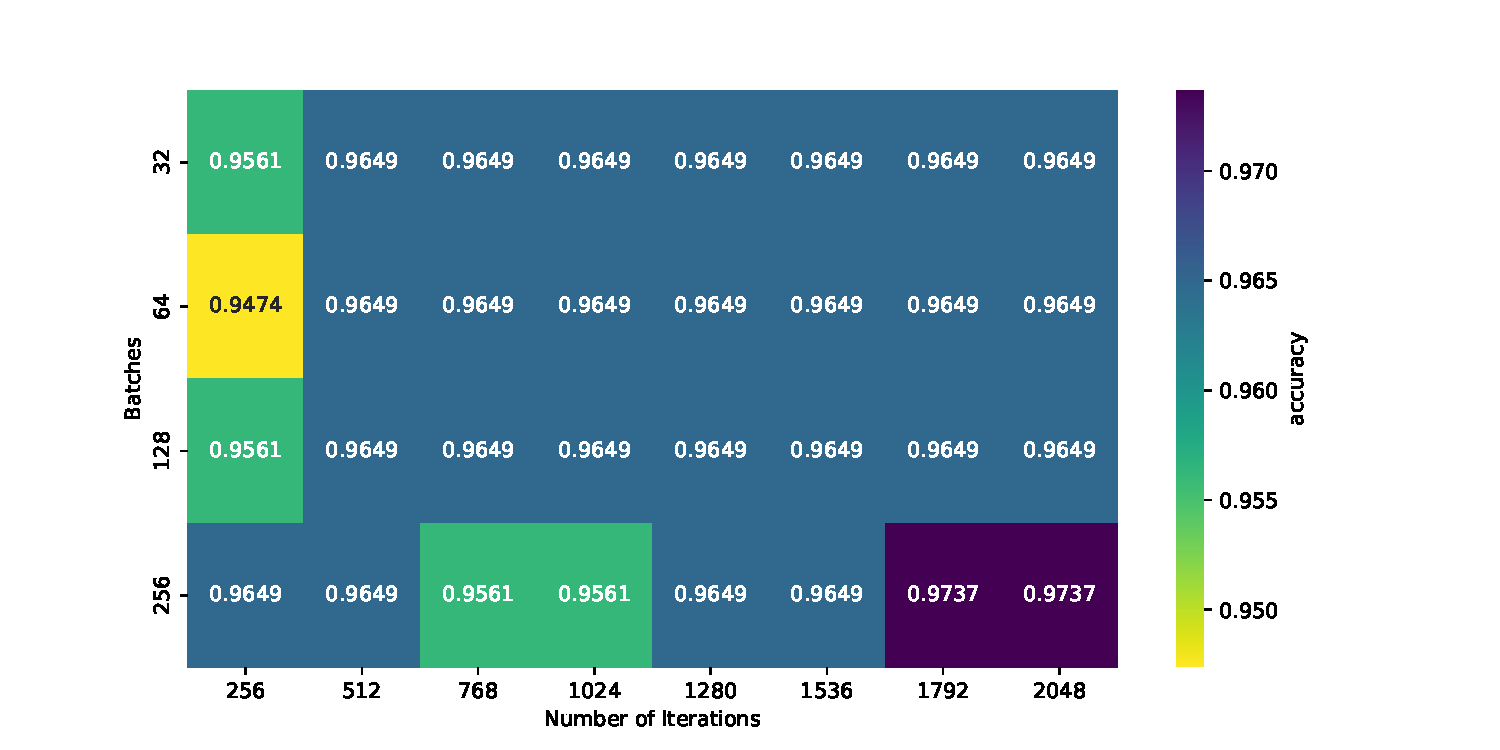
\includegraphics[width=1.0\linewidth]{Project 2/figures/class/NN_class_sigmoid_iterations_batches.pdf} 
    \caption{How the MSE for the MSE for the Wisconsin Breast Cancer data varies with the batches and epochs, using the Sigmoid function as an activation function. Hidden layers = 1, neurons = 25, $\eta$ = 0.1, l2=0.0. 
    }
    \label{fig: nn_iter_batch}
\end{figure}


\begin{itemize}
\color{white}
\item First item
\item Second item
\end{itemize}



\onecolumngrid
%\bibliography{ref.bib}
\end{document}